\documentclass[a4paper, 11pt]{article}

\usepackage[utf8]{inputenc}
\usepackage[swedish]{babel}

\usepackage{amsmath}
\usepackage{amsfonts}
\usepackage{amssymb}
\usepackage{graphicx}
\usepackage{float}
\usepackage{listings}
\usepackage{multirow}
\usepackage{fontenc}
\usepackage{wrapfig}

\usepackage[hidelinks]{hyperref}

%\usepackage{titlesec}
%\setcounter{secnumdepth}{4}

\usepackage[backend=biber,style=numeric,sorting=none]{biblatex}
\addbibresource{cites.bib}

\usepackage{caption}
\captionsetup[figure]{name=Figur}


\begin{document}

\begin{titlepage}
\newcommand{\HRule}{\rule{\linewidth}{0.5mm}}
\begin{center}

\textsc{\Large }\\[2.5cm]
\textsc{\LARGE Uppsala Universitet}\\[1.5cm] 

\HRule \\[0.3cm]
{ \huge \textup {Historiekunskapsspel med semi-automatisk frågehämtning och ett balanseringssystem för frågor}}\\[0.3cm]
\HRule \\[1.5cm]

\Large \textsc{Författare:}\\[0.5cm]
\large \textup{Alfred Yrelin}\\
\large \textup{Alfred.Yrelin.2125@student.uu.se}\\ [0.2cm]
\large \textup{Josef Svensson}\\
\large \textup{Josef.Svensson.8440@student.uu.se}\\[0.2cm]
\large \textup{Philip Åkerfeldt}\\
\large \textup{Philip.Akerfeldt.4987@student.uu.se}\\[0.5cm]

\large \textup{\textup{Institutionen för informationsteknolog}}\\
\large \textup{\textup{Uppsala Universitet}}\\[0.6cm]
\end{center}
~ \hfill
\center
~
{\Large \today}\\[2cm]
\vfill

\end{titlepage}

\newpage

\pagenumbering{gobble}
\begin{abstract}
Chronos är ett mobilspel utvecklat till Android som går ut på att rangordna historiska händelser bättre än motståndaren. Du kan spela mot antingen din kompis, eller mot någon okänd.
Varje spelare får en bunt händelser och den som kan relatera dessa till varandra och sätta dem i rätt ordning vinner. 

Chronos är inte bara ett roligt spel. Bakom användarens gränssnitt finns det ett intelligent system som anpassar spelet åt spelaren, för en maximalt rolig spelupplevelse. Spelet analyserar spelarens kunskapsnivå och anpassar händelserna i spelet för att matcha nivån. Serverapplikationen har också ett smart system för att automatiskt uppdatera spelet med nya frågor så att den erfarne spelaren aldrig får tråkigt.

Serverdelen är skriven i GO och använder Googles App Engine som plattform till stor del på grund av skalbarheten. Det intelligenta systemet balanserar frågorna och spelarna enligt Elo, ett system som används i många populära multiplayerspel.
\end{abstract}

\begin{abstract}
Chronos is a mobile game developed on the Android platform. The goal of the game is to arrange historical events in the correct order and to do it better than your opponent. You are able to play against either your friend or someone unknown. Each player is served a bunch of events and the one able to arrange them in most correct order is the winner.

Chronos is not just not a fun game. Behind the users interface there exists a intelligent system which adapts the game depending on the player, to get the most fun out of the game. The game analyses the players knowledge and adapts the questions against that. The server also has a system that automatically updates the database with new events so that the experienced player never gets bored. 

The serever is written in the language GO and it uses Google App Engine as platform mostly due to its scalability. The intelligent system adapts the questions with Elo, which is a system used in many popular multiplayer games.
\end{abstract}
\begin{center}
\textbf{Förord}\\
\textit{Tack till}
\end{center}
\newpage
\tableofcontents
\pagebreak

\pagenumbering{arabic}



\section{Inledning}
Vem vill inte kunna avgöra diskussioner med sina vänner med argumentet "Jag är i alla fall bäst på ..."? 
Att tävla är både en rolig och en social aktivitet. Oavsett om målet är att vinna eller bara ha kul så får deltagarna ofta en tävlingskänsla. Att kunna få en kombination av en tävlingskänsla och nöje är något som vi tror är att eftersträva i utvecklingen av mobila spel. Spel som exempelvis Quizkampen~\cite{quiz} och Wordfeud~\cite{wordfeud} besitter båda denna egenskap och det är därför vi tror att dessa spel har blivit så populära på marknaden~\cite{appsalesrating}. Vi som utvecklare tyckte att Quizkampen och Wordfeud hade lyckats väl med att designa spel som är enkla, roliga, estetiskt vackra. Dessa applikationer var även effektiva i den meningen att man som spelare lätt kan navigera sig i applikationen. Vi eftersträvade att skapa ett spel som besatt samma egenskaper och som kan framkalla samma tävlingskänsla som dessa spel. Vi har utvecklat ett spel som går ut på att ordna historiska händelser relativt till andra händelser. 

Applikationsutveckling för mobila enheter är ett spännande område som växer~\cite{IDC}, under sista kvartalet av 2014 hade Android 81,5\% av marknaden och av de enheter som såldes hade 76,6\% Android som operativsystem. Enligt Digi-Capital-Found~\cite{revenue} var även Android operativsystemet som gav högst intäkter för utvecklare som placerat sina applikation i någon form av applikationsmarknad, även om intäkter per nerladdning i iOS fortfarande var större.

Chronos har utvecklats till Android med en backend som drar nytta av Google App Engines skalbarhet för att ge applikationen möjlighet att växa i takt med att användarantalet ökar. För att vi inte skulle behöva söka och manuellt lägga in ett stort antal frågor har en semi-automatisk frågehämtare utvecklats. Detta system bidrar till att Chronos inte blir repetitivt och tråkigt för användarna. Frågehämtaren möjliggör att frågorna kan hämtas, skapas och läggas in utan att vi behöver ägna mycket tid åt dessa uppgifter. En annan sak som utvecklats för att spelet ska vara roligare för alla är ett balanseringssystem som gör att händelserna som ges till spelarna är anpassade efter spelarens kunskapsnivå.


\section{Bakgrund}
Den här sektionen ger en översiktlig beskrivning av spel och koncept som var starkt relaterade till utvecklingen av vår applikation. Bland annat beskrivs kort några applikationer som utvecklats till samma marknad. Det ges också en översiktlig beskrivning av dessa applikationer, koncept och spel som, på ett eller annat sätt, använts som inspiration vid utvecklingen av applikationen. 

\subsection{Kunskapsspel för mobiltelefoner}
Wordfeud och Quizkampen är två populära turbaserade multiplayerspel där Quizkampen har 45 miljoner användare globalt~\cite{quiz} och Wordfeud har 20 miljoner användare~\cite{wordfeud}. Dessa spel gör det möjligt att utmana vänner eller slumpmässiga personer på en match som spelas i omgångar. När en spelare spelar sin omgång får motståndaren vänta på sin tur. Denna spelmekaniken gör att en match skulle kunna pågå i flera dagar.

Det intressanta med just de här applikationerna är deras upplägg. Wordfeud och Quizkampen är egentligen ganska olika men den övergripande strukturen är densamma. Eftersom båda dessa appar har visat sig vara populära så tror vi att samma typ av övergripande struktur är något som fungerar bra i utvecklingen av mobilspel. Quizkampen och Wordfeud är turbaserade spel vilket innebär att medan ena spelaren gör sitt drag så måste den andra spelaren vänta. Det här upplägget skapar en förväntan hos den väntande spelaren eftersom hen dels vill veta vem som gjort bäst ifrån sig men också för att hen vill göra sitt nästa drag. Förväntan är bra eftersom det höjer spelarens upplevelse av spelet. Varje gång spelaren tar upp sin telefon så \textit{hoppas} den att motspelaren har svarat. Det här innebär att spelaren associerar en positiv händelse med spelet och risken att spelaren tröttnar minskar.

Eftersom det turbaserade upplägget är ett väldigt bra upplägg som förhöjer förväntan i spelet så anammar även Chronos det upplägget. 

\subsubsection{Quizkampen}
Quizkampen~\cite{aboutquiz} är ett frågesportsspel där spelarna svarar på frågor under sex rundor med tre frågor i varje runda. Båda spelarna svarar på samma frågor varje runda.  Inför varje runda slumpas tre kategorier fram där någon av spelarna får välja en kategori för den aktuella rundan. Valet av kategorier är något som spelarna turas om att göra varannan runda. Matchen avslutas när sista rundan är spelad och det är även då en vinnare koras beroende på vem som har flest poäng. 

\subsubsection{Wordfeud}
Wordfeud~\cite{aboutwordfeud} är ett spel där en match utspelas mellan två personer. Varje spelare får en liten mängd bokstäver som är gömd för motspelaren. Spelet går sedan ut på att fläta samman ord på det givna spelbrädet med hjälp av bokstäverna. Målet är att få så många poäng som möjligt och detta kan man uppnå tack vare att varje bokstav är värd en viss poäng. På så sätt kan man genom att använda svårare bokstäver och skapa längre ord få mer poäng. 

\subsection{Sällskapsspel med fokus på kunskap} \label{nardada}
Sällskapsspel har länge varit och är än idag ett populärt sätt att umgås på~\cite{bradspelspop}. Sällskapsspelet \textit{När då då?}~\cite{nardada} är ett spel som bygger på ett relativt enkelt koncept. Spelarna turas om att placera ut händelser på sin egen tidslinje och får poäng om händelserna är korrekt utplacerade i förhållande till varandra. Varje tur för en spelare går till så att spelaren får en händelse uppläst för sig och sedan ska spelaren välja en plats på sin tidslinje att lägga händelsen på. Om spelaren lägger händelsen fel så är turen avslutad och spelet fortsätter till nästa spelare. Däremot, om händelsen är korrekt placerad får spelaren välja att antingen försöka placera en händelse till, eller att avsluta och säkra sina redan placerade händelser. Skulle spelaren förlora efter att ha placerat flera händelser samma runda så försvinner alla händelser i den rundan. Spelet fortsätter tills dess att någon spelare har lyckats placera åtta händelser korrekt, då spelas rundan klart och den spelare med flest poäng vinner.\\

Spelkonceptet är som sagt ett enkelt sådant men det är också kraftfullt i den meningen att det lyfter fram vissa begär hos spelarna. Ett av begären är att man vill överkomma problem som ställs av antingen spelet själv eller motspelarna. Detta är en av faktorerna som gör den typen av spel så populära~\cite[sid 3--4]{psykologi}. En annan intressant faktor i det här spelet är girigheten som infinner sig när spelaren har möjlighet att välja mellan att fortsätta sin tur eller att säkra sina frågor. Det är en viktig del av spelet som kan förändra väldigt mycket. En spelare har möjlighet att nästan vinna på sin första runda, för att sedan förlora alla sina händelser för att den sista placerades fel. Det här ökar spänningen i \textit{När då då?}.

\subsection{Automatisk informationshämtning}
För spelets överlevnad är det viktigt att frågorna aldrig tar slut. Det är också viktigt att frågorna håller hög kvalitet och att inga missförstånd uppkommer. Eftersom internet består av fantastiskt mycket information som går att relatera till årtal så vore det en bra idé att på något vis dra nytta av den här informationen. Man skulle kunna tänka sig att flera personer arbetar aktivt under en lägre tid med att sammanställa händelser och manuellt fylla en databas med dessa. Fördelen med detta vore att en hög kvalitét nästan kan garanteras (förutsatt att personerna som sammanställer händelserna har en känsla för det). Nackdelen är att det tar mycket tid att sammanställa informationen manuellt.

På grund av detta vore det bra med ett system som automatiskt sammanställer händelser utifrån den historiska data som redan finns tillgänglig på internet. För att främja systemets tillförlitlighet och kvalitéten på de producerade frågorna begränsas det automatiska systemet till att endast hämta information från Wikipedia. Tillförlitligheten och kvalitéten kan höjas med den här begränsningen eftersom utvecklarna har större möjlighet att göra antaganden om hur informationen som ska genomsökas (Wikipedia) ser ut. Det här gör att filtreringen blir lättare att konstruera samt att risken för fel blir mindre.

Wikipedia har några olika standardlayouter på sina informationssidor och en av dessa layouter är en punktlista med årtal. 

%\begin{figure}[H]
%	\begin{centering}
%	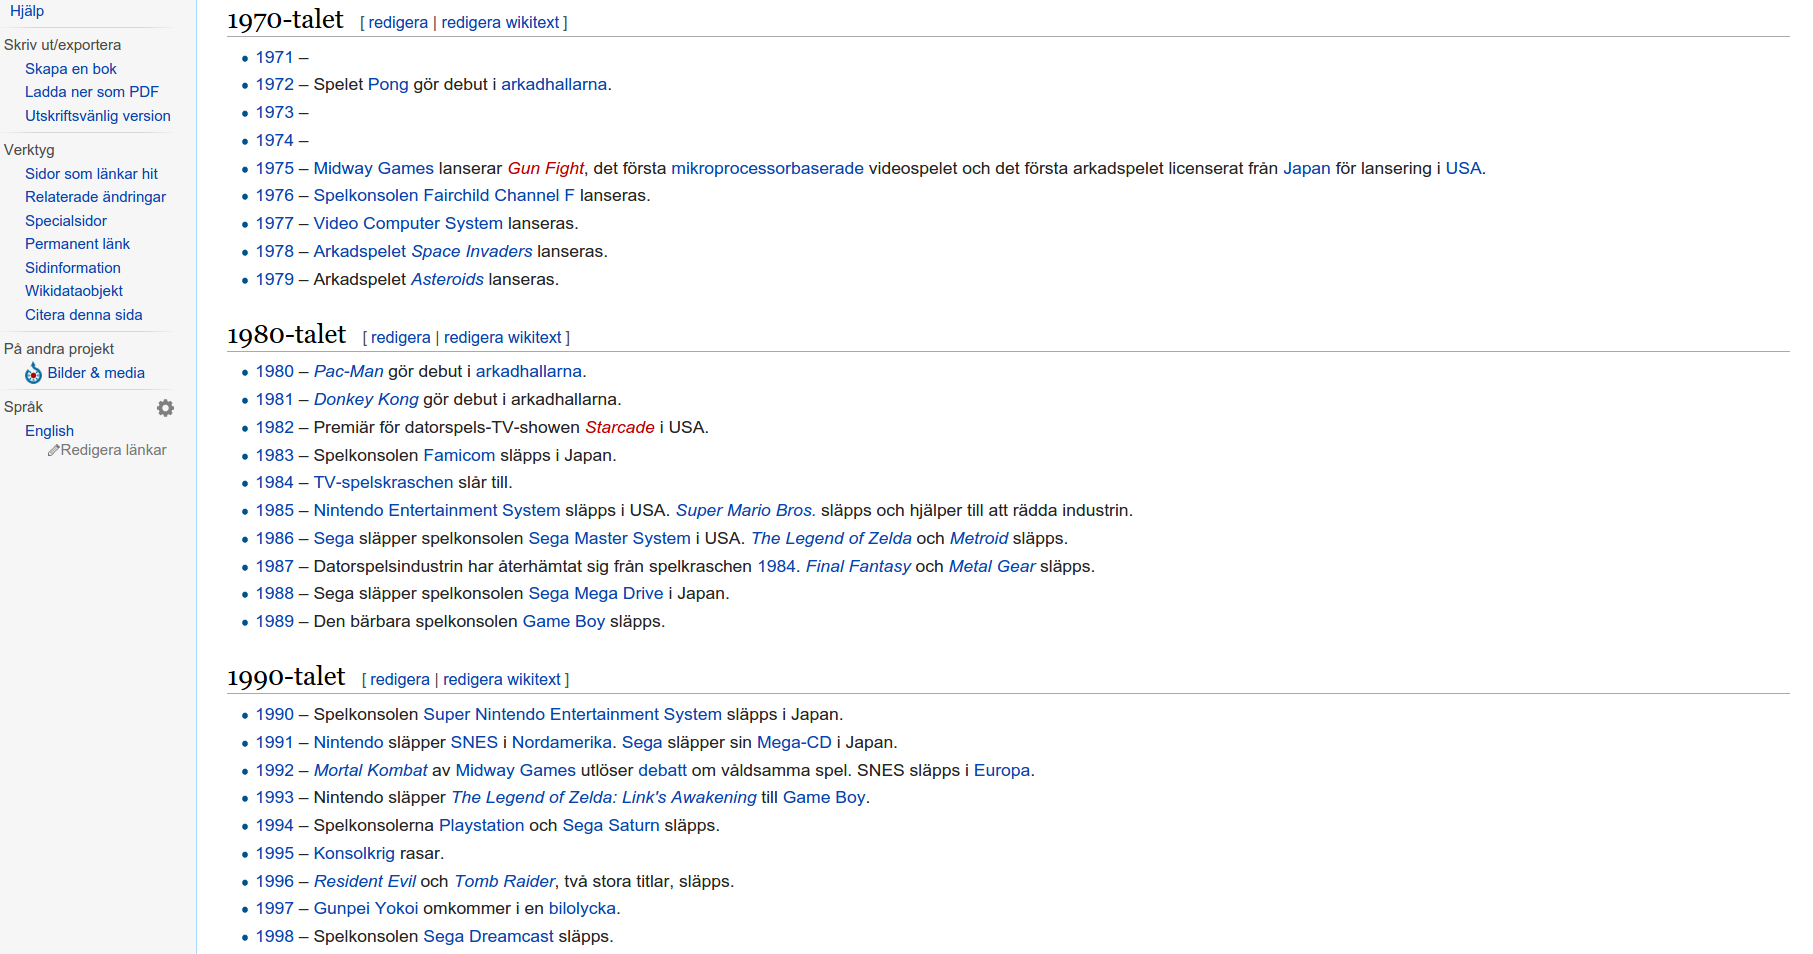
\includegraphics[width = \textwidth]{Listbild.jpg} 
%	\end{centering}
%	\caption{\textit{Exempel av hur Wikipedia illustrerar listsidor.}}
%\end{figure} 

Informationen i den här typen av lista presenteras alltid likadant och förekommer på många undersidor inom olika ämnen på Wikipedia. Varje händelse och årtal presenteras som punkter, likt denna:\\

	1993 – Nintendo släpper The Legend of Zelda: Link's Awakening till Game Boy.\\

Eftersom presentationen är konsekvent, med ett bindestreck som avskiljer årtal och händelse är inhämtning av information från de här sidorna enkel att automatisera.

\subsubsection{Webcrawler}

En webcrawler är ett system som automatiskt söker igenom webbsidor. Syftet med en webcrawler är att hämta information från sidan som söks igenom samt dess länkar, för att sedan göra samma sak på alla undersidor och så vidare. Googles \textit{Googlebot}~\cite{googlebot} är ett exempel på en webcrawler som syftar till att indexera hela webben för att göra den sökbar via Googles sökmotor, www.google.se.

Den automatiska informationshämtningen i Chronos bygger på den här principen. I det här begränsade fallet söks endast utvalda Wikipediasidor igenom, men syftet är detsamma, att spara information som systemet hittar. 

\subsection{Balansering}
Begreppet balansering syftar på tekniker för att göra spelet så jämnt och rättvist som möjligt samtidigt som det är roligt. Ett spel blir roligast när man spelar mot likvärdiga motståndare och får frågor som är något utmanande men inte helt omöjliga. Det ska inte vara för lätt att vinna och inte heller för svårt. Det finns två huvuddelar i Chronos som är möjliga att anpassa för att justera svårighetsgraden för spelaren. Det ena är händelsernas svårighet, det vill säga, hur pass troligt det är att spelaren vet när händelsen ägde rum. Det andra är motståndarens skicklighet.


\section{Projektbeskrivning}
Denna sektion lägger betoning på varför applikationen utvecklades. Vad som var våra mål med projektet, motivation för utvecklingen, vilka avgränsningar som gjordes, vilka krav vi ställde på applikationen, vilka tekniska problem vi var tvungna att överkomma samt vad som gjorde Chronos unikt i förhållande till konkurrenterna.

\subsection{Syfte}
Det var projektets syfte att utveckla och distribuera en spelapplikation för mobila enheter som använder plattformen Android. Applikationen skulle ge flera användare möjlighet att interagera och spela med varandra samtidigt.

Spelet som utvecklats går ut på att två användare får tävla om vem som har bäst koll på när olika historiska händelser ägde rum. Varje spelare får ett antal händelser som den sedan ska sortera i kronologisk ordning. Spelaren som sorterar flest händelser rätt vinner. Förutom rent nöje så kan spelet användas i utbildningssyfte. Detta i den meningen att det ger användaren en ypperlig möjlighet att förbättra sina kunskaper om historien.

\subsection{Mål}
Det fanns fyra stora delar i det här projektet som kan ses som projektets primära fokuspunkter. Målet vi hade för avsikt att uppnå är en mobilapplikation i form av ett spel. Spelet skulle köras på en server som har för uppgift att sköta all kommunikation mellan klienten och sig själv. En av de primära fokuspunkterna för spelet var att implementera en semi-automatisk informationshämtare som skulle fylla på spelets databas med nya frågor. Att informationshämtningen är semi-automatiskt betyder att ett steg i informationshämtningen kräver mänsklig interaktion. Interaktionen krävdes för att godkänna frågorna till databasen och detta är en uppgift som administratörerna utför. 


\subsubsection{Mobilapplikation}
Vi strävade mot att utveckla en mobilapplikation till Android. Applikationen är det enda som användaren i slutändan ser och därför att kvaliteten av gränssnittet var extra viktigt att fokusera på i utvecklingen. 

Applikationen till Android skrevs i Java och gränssnittet skrevs med hjälp av XML ~\cite{xml}. 

\subsubsection{Server}
För att flera spelare skulle kunna interagera med varandra så behövdes det en server. En server möjliggjorde även att frågorna i spelet kunde uppdateras kontinuerligt under applikationens exekvering.

Servermjukvaran skrevs i programspråket Go~\cite{golang} och körs på Googles molntjänst App Engine.

\subsubsection{Automatisk informationshämtning}
För att spelet skulle bli så intressant som möjligt behövdes en stor bredd på frågorna som skulle lagras i spelets tillhörande databas. Ett sätt att skapa många frågor snabbt var att utveckla mjukvara som kunde hämta information och från denna information skapa nya frågor automatiskt. 

Målet med den automatiska informationshämtningen var att skapa ett delsystem som läste in delar av en hemsida, som följer en viss struktur, för att hitta nödvändig information. Systemet skulle sedan koppla samman årtalen och händelserna från hemsidan automatiskt. Systemet behövde också ett gränssnitt för att ge administratörerna ett snabbt sätt att korrekturläsa frågorna innan de godkändes och skickades vidare till spelet.

\subsection{Frågeställningar}

\subsubsection{Tekniska problem}
Det fanns vissa delar i det här systemet som var mer avancerade att lösa än andra delar. En lista av följande utmaningar presenteras nedan.
\begin{itemize}
\item Eftersom applikationen på något sätt skulle hämta information och konstruera frågor på ett semi-automatiskt sätt var det ett måste att utveckla ett sådant system. En svårighet i detta var att se till att systemet blev tillräckligt smart för att lyckas läsa en informationskälla och ta ut den eftertraktade informationen på rätt sätt.
\item Det behövdes en relativt stor databas för att lagra både användare och frågor för spelet. Det här var något som vi inte hade arbetat med på en stor skala förut. Hur skulle man lagra informationen på ett sätt som var både effektivt lagringsmässigt samt snabbt och enkelt för servern att hämta?
\item Det krävdes nätverkskommunikation med säkerhet och användaridentifiering. App Engine som användes vid stora delar av utveckling hade användbara funktioner som uppfyllde vissa av våra krav men inte alla. Hur skulle vi lyckas tillgodose användarna med en säker applikation?
\item Spelet skulle anpassa svårighetsgraden automatiskt vilket innebar att någon form av balansering krävdes. Tanken var att frågorna skulle ha en svårighetsgrad som justerades automatiskt beroende på hur ofta de placerades rätt. Här var vi tvungna att ta hänsyn till hur resten av tidslinjen såg ut vid tillfället. Hur skulle detta utvecklas på ett tillräckligt effektivt och rättvist sätt för applikationen och användarna.
\item Det fanns ett behov att utveckla ett system för att rangordna spelare i någon slags topplista. Hur skulle detta ske och hur skulle rangordningen bestämmas utifrån spelets mekanik? 
\end{itemize}

\subsection{Relaterat arbete}

\subsubsection{Historiekampen} \label{Historiekampen}
Det finns ett spel för iOS, \textit{Historiekampen} ~\cite{historiekampen} som också handlar om att lägga in händelser korrekt på en tidslinje. En nackdel som den befintliga iOS-versionen har är att användaren endast ser årtal på sin tidslinje, och inte vilka händelser som ligger där.

Historiekampen är ett spel som konceptuellt sett liknar sällskapsspelet \textit{När då då?} väldigt mycket. En spelares tur går till så att den först får en händelse som skulle placeras på spelarens tidslinje. När första frågan presenterades fanns det en årtalsreferens utlagd på tidslinjen som den första händelsen ska placeras före eller efter. När nästa fråga presenteras finns det två referenser (den första plus årtalet för frågan som precis placerades) och så vidare.\\ 
Historiekampen har valt att använda konceptet med kombinationspoäng vilket implicerade att spelaren kan få flera poäng under en runda om den placerar ut flera händelser korrekt efter varandra. Spelaren är tvungen att placera minst \underline{en} händelse och kan få maximalt tio händelser att placera ut. Om spelaren placerar första händelsen fel avslutas rundan. Placerade spelaren istället händelsen rätt ställs den inför ett val med två alternativ: antingen avsluta sin runda och på så sätt låsa sina poäng, eller fortsätta att få händelser att placera ut i förhållande till de tidigare händelserna. Detta val gör spelaren efter varje rätt placerad händelse. Spelaren kan med andra ord välja själv om den vågar fortsätta eller om den vill vara försiktig och behålla sina välförtjänta poäng. En duktig spelare kan välja det senare alternativet och bygga upp sin kombo fram tills dess att den femte frågan är ställd. När den femte frågan är ställd får spelaren en fråga om \textbf{när} den femte händelsen ägde rum. Om spelarens svar är nära det rätta årtalet får spelaren fortsätta rundan med sin uppbyggda kombo av poäng. Om årtalet var fel förlorar spelaren sina tidigare poäng men kan fortsätta få händelser att placera ut i förhållande till de tidigare händelserna. Vid en perfekt runda kan en spelare få totalt tio poäng.\\

En av utvecklarna av Historiekampen vid namn Viktor Ström kontaktades av Chronos utvecklare 12 Maj 2015. Efter förfrågan beskrev Viktor hur applikationen fungerade. Viktor beskrev att frågorna/händelserna till applikationen hade skapats manuellt vilket tog sin tid men var något man var tvungen göra för att frågorna skulle uppnå en hög kvalitet. Vilka händelser som spelaren fick var helt slumpmässigt men båda spelarna fick samma händelser i samma ordning. När en vän utmana så markeras händelserna i den matchen som ``använda'' i spelarens app och skulle inte återkomma förrän hen gått igenom samtliga händelser. Spelaren kan dock få samma händelser om någon annan utmanar hen eftersom händelserna inte nödvändigtvis är markerade som använda i motståndarens app. 
Viktor nämnde även att svårighetsgraden på matcherna kunde variera mycket. Vissa matcher är lätta och vissa svåra, men eftersom spelarna alltid får samma händelser i samma ordning så tycker han att svårighetsgraden spelar mindre roll eftersom det är ``lika för alla'' -- (Viktor Ström, personlig kommunikation, 12 Maj, 2015). 


\subsubsection{Balanseringsteori}
En viktig aspekt i det här projektet var att rangordna spelare i förhållande till varandra för att skapa mer rättvisa matcher. Den här problematiken fanns det redan många som hade funderat på och de flesta större spel använder sig också av något system för balansering. Två etablerade system är Elo och Glicko, varav Elo är det som har implementerats i det här projektet.

Elo är ett system som förutser hur stor del av en mängd spelade matcher som bör vinnas av vardera spelare. Detta baseras på en den svårighetsnivå respektive spelare har. Det här systemet justerar, efter en match, poängen enligt förutsättningarna som finns beskrivna ovan. Eftersom en lägre rankad spelare får fler poäng vid vinst mot en högre rankade spelare rättar systemet på sikt sig självt, vilket innebär att spelarna faktiskt får den nivå de förtjänar.

Elo-systemet fungerar enligt följande. Varje spelare får en initial Elo-poäng på 1000. Denna justeras sedan beroende på utfallet av en match i förhållande till det förväntade utfallet. Det förväntade utfallet beräknas:

$$E_A = \frac{1}{1+10^{(R_B-R_A)/400}}$$

Där $E_A$ är den förväntade andelen matcher som spelare A borde vinna. Är värdet till exempel 0.84 så innebär det att 84\% av matcherna borde vinnas av spelare A enligt nuvarande Elo-poäng. $R_B$ är spelare B:s nuvarande Elo-poäng och $R_A$ är spelare A:s nuvarande poäng.

När det förväntade utfallet har beräknats så justeras sedan spelarnas Elo-poäng enligt formeln:

$$R'_A = R_A + K(S_A-E_A)$$

Där $R'_A$ är spelare A:s nya Elo-poäng, $R_A$ är spelare A:s Elo-poäng innan matchen, $S_A$ är det faktiska utfallet av matchen och $E_A$ är det förväntade utfallet. K-värdet är en skalningsfaktor som justerar hur mycket poängen justeras vid varje vinst/förlust.

Ett räkneexempel med spelare A, 1300 poäng, och spelare B 1000 poäng, där A vinner:

$$0.849 = \frac{1}{1+10^{(1000-1300)/400}}$$
$$ R'_A = 1300 + 16(1-0.849) = 1302.416 $$
$$ R'_B = 1000 + 16(0-0.849) = 997.584 $$

I det implementerade balanseringssystemet används Elo-modellen för att beräkna spelarnas erfarenhetspoäng. Elo är ett system som utvecklades av Arpad Elo och började användas redan på 60-talet ~\cite{elo}. Systemet var först och främst utvecklat för att ranka schackspelare, men har sedan dess uppkomst även applicerats på många andra spel. Eftersom Elo-systemet är förhållandevis gammalt och möjligheten till datoriserade beräkningar blivit större sedan 60-talet, finns det mer avancerade system att använda sig av idag. Ett annat system som utvecklades i syfte att vara en förbättring av Elo-systemet är ett system kallat Glicko ~\cite{chessratings}. Skillnaden mellan Elo och Glicko är att Glicko också har ett värde för hur väl uppdaterad spelarens erfarenhetspoäng är. Det här innebär att spelaren har ett erfarenhetspoäng, säg 2000, samt ett trovärdighetspoäng, till exempel 100. Ju högre trovärdighetspoäng spelaren har, desto mindre exakt är erfarenhetspoängen. Erfarenhetspoängen har enligt systemet en +/- diff på dubbla trovärdighetspoängen. I nyss nämnda exempel innebär detta att spelaren har en erfarenhetspoäng på 1800-2200. Trovärdighetspoängen justeras bland annat baserat på hur länge sedan det var spelaren spelade förra gången, samt hur många matcher spelaren spelat totalt. Ju fler matcher totalt och ju närmare i tid förra matchen var, desto lägre trovärdighetspoäng har spelaren.

Både Elo och Glicko används idag och det verkar vara svårt att avgöra om Glicko verkligen är bättre än Elo ~\cite{stackchess}. Ett faktum som finns är i alla fall att Glicko kräver mer information för att kunna fungera. En faktor som Glicko behöver men inte Elo är en tidsvariabel som har reda på hur länge sedan det var spelaren spelade sin förra match ~\cite{glickoex}. Det här gör att mer data behöver lagras i databasen, vilket är negativt ur kapacitetsperspektiv.

\subsubsection{Chronos spets}
Chronos liknar Historiekampen (avsnitt \ref{Historiekampen}) och \textit{När då då?} (avsnitt \ref{nardada}) rent konceptuellt. Uppgiften som spelarna utför i vår applikation och uppgifterna som skulle utföras i Historiekampen liknade varandra mycket. I både Historiekampen och Chronos är det spelarens uppgift att placera ut händelser rätt på en tidslinje. Spelmekaniken är dock annorlunda i vår applikation då varje match och varje runda behandlades annorlunda. I Chronos får varje spelare ett paket med sex frågor för varje runda. En av dessa sex frågor agerar som referenshändelse på tidlinjen. Frågorna presenteras för spelaren en i taget och det är sedan spelarens uppgift att placera dessa i rätt ordning. En spelare får ett poäng per korrekt utplacerad händelse och kan på så sätt få maximalt fem poäng från de korrekt placerade händelserna. Om en spelare lyckas få en perfekt runda, där alla händelser placerades rätt, får den ett extra poäng vilket resulterar i en total summa av sex poäng. Likt Historiekampen avslutas en runda när en spelare har placerat en händelse fel. Det som skiljer vår applikation i denna aspekt är vid fallet då en spelare har tjänat ihop poäng från tidigare händelser. I Historiekampen förlorar spelaren alla sina tidigare poäng om den svarar fel medan i vår applikation får spelaren behålla sina poäng. Oavsett om spelaren lyckats placera ut alla händelser rätt eller inte så går turen, efter fem frågor, över till motståndaren. När fem rundor har spelats vinner den spelare som har svarat rätt på flest frågor totalt.  

En viktig detalj som skiljer Chronos från Historiekampen är faktumet att spelaren ser beskrivningen av händelserna som spelaren placerat tidigare istället för bara årtalen. Vid avslutad runda visas även de korrekta årtalen för händelserna så att spelaren vet vilken ordning som hade varit den korrekta. Chronos handlar med andra ord mer om att relatera händelser till varandra (dog Palme efter andra världskriget?) istället för att veta vilket årtal det skedde.

Med den semi-automatiska frågehämtaren, som kan anpassas för olika informationskällor, är det enkelt för administratörerna att hämta nya händelser. Databasen med händelser kan på så sätt expandera snabbt vid behov. Detta är något som skiljde oss från Historiekampen där alla frågor matades in manuellt. \\
Applikationen balanserade även händelsernas svårighetsgrad kontinuerligt efter varje match vilket bidrog till att alla spelare tilldelades händelser som passade deras aktuella kunskapsnivå. Balanseringen ansvarade även för att se till att slumpade matcher skulle ske mellan spelare av ungefär samma kunskapsnivå. En novis skulle med andra ord inte behöva möta en mästare. Balanseringen i spelet kan även byggas ut och göras mer avancerad om användarna skulle ge kritik på hur frågorna rankades. Det finns egentligen inga gränser för hur avancerad balansering kunde göras vilket är en stor fördel som skiljer oss från konkurrenterna.

\subsection{Motivation}
Det finns många mobilspel som handlar om att två personer möts och mäter sina färdigheter inom ett visst område. Exempel på sådana applikationer är Quizkampen och Wordfeud som båda toppar säljlistorna för Androidspel~\cite{appsalesrating}. Dessa spel följer en ganska enkel struktur och den bygger på att två personer kan möta varandra för att sedan svara på frågor eller lägga ord korrekt. På detta sätt får spelarna poäng som sen avgör vinnaren mellan de tävlande. Enligt säljstatistiken~\cite{appsalesrating} är detta koncept något som är attraktivt för många användare. Chronos kombinerar koncepten från Quizkampen och Wordfeud i den mening att spelare på sätt och vis ska svara på frågor samt att lägga in saker på sin rätta plats. 

En liknande version av Chronos har också visat sig vara populär i form av sällskapsspel (\textit{När-då-då?})~\cite{nardada}. Detta var en av anledningarna till att förhoppningarna var höga att även vår applikation ska bli populär på marknaden. Det finns för tillfället ingen variant av det här spelkonceptet till Android vilket ger Chronos stora möjligheter att lyckas.

\subsection{Avgränsningar}
Någon applikation för Windows phone och iOS skulle inte utvecklas parallellt med applikationen för Android. Versioner av applikationen för iOS och Windows phone fanns som en eventuell fortsatt utveckling efter Androidapplikationen. Detta på grund av att ett större fokus på en bra applikation till Android prioriterades. Vi valde att utveckla applikationen för Android 4.4 och uppåt vilket betyder att äldre modeller inte är kompatibla med applikationen.
Vi ville även utveckla ett par olika kategorier för händelserna men dessa planer sköts upp tills vidare. Detta beslut togs för att tiden inte tillät oss förverkliga vår planering.

I planeringen för applikationen fanns det många funktioner som skulle vara roliga och användbara att implementera, men inför projektet var det några funktioner som ansågs vara viktigast att ha med. Den viktigaste funktionen var att kunna hitta och spela en match. En funktion för att hitta och hantera vänner man har i spelet och även en funktion för att kunna se statistik över matcherna man spelat mot en vän. Dessa funktioner behövde så klart även implementeras på servern.

\subsection{Krav}
Systemet skulle klara av många spelare samtidigt men endast två per match. Något tak för antalet användare var inte bestämt. Tack vare den otroligt solida grunden för skalbarhet som projektet stod på skulle ett mål för önskat antal användare vara lätt att bestämma. Eftersom App Engine användes för servern så skulle det inte bli några problem med den enkla förklaringen att det är en tjänst som automatiskt skalar med hänsyn till belastningen~\cite{appenginescalability}. 

Informationssökaren skulle tillsammans med den administrativa kontrollen ge frågor som håller hög kvalitet. Hög kvalitet innebär frågor som är relevanta och som följer den strukturen som vi hade tänkt oss. Frågorna skulle vara lätta att läsa, förstå och samtidigt befinna sig i det breda spektrumet av svårighetsgrader som spelet skulle ha. Frågehämtaren skulle också vara så pass bra att den administrativa kontrollen gick fort och att så lite som möjligt behövdes korrigeras efter att frågorna hade samlats in. För att applikationen inte skulle kännas alldeles för repetitiv skulle det finnas många frågor som dessutom var av varierande kategori. Det skulle även finnas minst 1000 frågor i spelet.

Designen av applikationen var något som var väldigt viktigt för oss. Kravet i början var att ha en intuitiv, responsiv och snygg design. Eftersom applikationen gjordes för Android skulle den också följa dess designmönster, Material Design~\cite{MaterialDesign}.

\section{Implementation}
Den här sektionen beskriver hur de målsatta delarna implementerades i applikationen samt metoderna som användes för att lyckas med detta. Applikationens systemstruktur och dess innefattande delar förklaras och illustreras. Det finns även en grundlig genomgång av hur applikationen ser ut samt hur den fungerar, både för användare och systemadministratörer.

\subsection{Metoder}
Ett antal olika verktyg användes för att möjliggöra detta projekt. För utvecklingen och simuleringen av Androidapplikationen användes Android Studio~\cite{androidstudio}. Detta är ett kraftfullt verktyg som på ett smidigt sätt bland annat kan simulera applikationen i olika valbara miljöer i form av layouts för olika mobiltelefoner.\\
Google App Engine användes lokalt för att simulera serverapplikationen. När tidsperioden för den första testningen var över användes fortfarande App Engine men då i Googles moln istället för lokalt. App engine var ett värdefullt verktyg i vår utveckling med den enkla förklaringen att de tjänster som erbjöds när man utvecklade och körde sina applikationer via denna motor var otroligt värdefulla. Det var bland annat lätt att underhålla applikationen och skala upp när trafik och data krävde det~\cite{googleappengine}. 

% Det här stämmer inte
%
%Den primära källan för information till frågorna var under utvecklingsfasen Wikipedia men denna ersattes mot andra informationskällor vid ett senare skede. Detta förekom innan produkten färdigställdes.\\ 
%Valet att inte använda Wikipedia som informationskälla i den slutgiltiga versionen av applikationen berodde på dess tvivelaktiga rykte som en pålitlig källa. Wikipedia trovärdighet har länge diskuterats och det finns många rapporter som har undersökt dess trovärdighet. Att använda Wikipedia för att bekanta sig med ett ämne är, enligt oss, fullt acceptabelt men borde lämpligtvis granskas kritiskt innan den användes som källa. Relationen mellan processerna att skapa och redigera artiklar på Wikipedia anses vara en ledande faktor till denna osäkerhet. Detta beror mycket på att hemsidan följer strukturen \textit{editable-by-all} vilket innebär att vem som helst kan ändra artiklar och på så sätt vinkla artikelns innehåll på ett eller ett annat sätt. Detta implicerar såklart inte att alla artiklar har råkat ut för detta öde men det bidrar till en viss osäkerhet vid användandet av denna hemsida som källa vid vetenskapliga rapporter ~\cite[sid 27--34]{wikipediacred}.

\subsubsection{Google App Engine} \label{Google App Engine}
Google App Engine är en \textit{Platform as a service}, vilket är en servicemodell för molntjänster. Det bygger på att utvecklare skapar en programvara med hjälp av färdigbyggda bibliotek och verktyg som leverantören tillhandahåller. Den utvecklade produkten kan sedan köras vid Google App Engine. Servern som vi byggde i App Engine kördes på Googles infrastruktur och var uppbyggt så att antalet användare för applikationen kunde utökas obegränsat. Flera stora företag använder sig av App Engine när deras produkter lanserades där några exempel av större företag var Coca Cola, Rovio och Best Buy~\cite{googleappenginecustomers}. 

\subsection{Systemstruktur}

\begin{figure}[H]
	\begin{centering}
	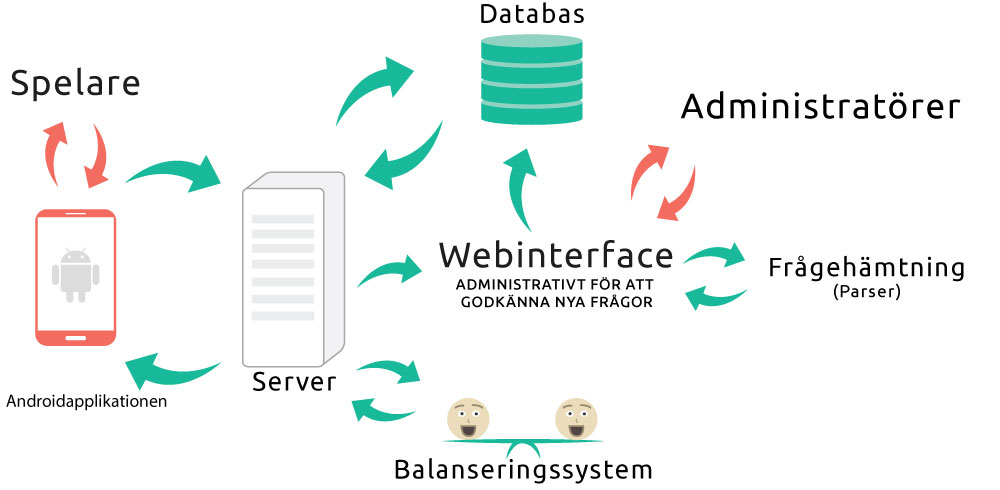
\includegraphics[width = \textwidth]{systemstruktur2.jpg} 
	\end{centering}
	\caption{\textit{Illustration av systemstrukturen}}
\end{figure} 

Hela systemet består av fem delar som interagerar med varandra. Närmast spelaren finns klienten vilket är det enda som spelaren ser. Klienten är byggd för Android som en mobilapplikation. Mobilapplikationen interagerar i sin tur med serverns API. Servern fungerar som en länk mellan klienten och resten av delarna i systemet.

På serversidan av systemet finns en semiautomatisk frågehämtare, ett balanseringssystem och en databas. Frågehämtaren hanterar automatisk generering av frågor och balanseringssystemet justerar svårighetsnivåerna på spelarna och frågorna för att maximera spelupplevelsen.

\subsubsection{Androidapplikationen}
Androidapplikationen, klienten i systemet, var själva spelet som utvecklades. Det var den del av systemet som användaren interagerade med båda visuellt och funktionellt.

När det är den aktuella spelarens tur får hen en chunk med sex frågor och dess svar (årtal) från systemets server. Svaren är gömda för användaren under rundans gång och används endast av klienten för att rätta svaren från spelaren. När spelaren är färdig med sin runda och klienten har rättat svaren så skickas dessa tillbaka till servern där de lagras i matchens historik. 

\subsubsection{Server}
Klienten kommunicerar med en server som körs i Google App Engine. Servern är utvecklad i programspråket Go (Golang)~\cite{golang}. Anledningen till att vi valde att skriva servern i Go var för att det, enligt oss, var ett simpelt språk med en syntax som liknade andra språk som vi hade använt tidigare. Servern agerar även som en brygga mellan klienten och den databas som används. När klienten kräver nya frågor till spelet kommunicerar servern med databasen. Databasen skickar frågor till servern som i sin tur skickar vidare till klienten. Utöver kommunikation till klienten och databasen används även servern för att köra crawlern som är den semi-automatiska informationshämtaren. Servern har också som uppgift att med jämna mellanrum köra fråge- och användarbalanseringssystemet som justerar svårighetsgraden för frågorna respektive spelarna i systemet. 

\subsubsection{Databas}
Databasen som servern kommunicerar med körs, likt servern, i App engine med biblioteket \textit{datastore}. Datastore~\cite{datastore} är Google App Engines egna bibliotek för hantering och lagring av data vilket innebär att systemet, utan vår assistans, hanterar all datalagring. Datastore har flera egenskaper som bidrar till en enklare utveckling av resterande delar för projektet. Med tanke på att Datastore är ett bibliotek från App Engine så medföljer dess skalbarhet som skalar beroende på behovet. Med Datastores inbyggda hjälpmedel för redundans kan data lätt replikeras till flera datacenter om det skulle behövas. \\
Datastore hanterar datalagring med både SQL och NoSQL. För den som inte är bekant med NoSQL så är det en alternativ design för databaser som skiljer sig från SQL-databaser~\cite{nosql}. Marknaden som existerar idag är vad som kan kallas för en \textit{Big Data Reality} som kännetecknas av den enorma mängd data som måste hanteras av dagens databaser. Designen för NoSQL utvecklades för att möta kraven som ställdes av dagens \textit{Big Data Reality}. NoSQL utvecklades för att bidra med en enklare design och lättare tillgänglighet. Det är mest strukturella skillnader mellan NoSQL och vanliga relationsdatabaser. Det betyder att vissa operationer är lättare och mer effektiva att utföra i NoSQL medan andra är snabbare i vanliga relationsdatabaser~\cite[1--3]{nosqlfacts}. NoSQL används alltmer av applikationer som måste hantera stora mängder data men också websystem som ska exekveras i realtid~\cite{nosqlcloud}. Egenskaperna som NoSQL besitter passar för vår applikationen då ett tak för antalet användare inte var satt samt att vi önskade att exekvera i realtid.

Med Datastore behövde vi inte oroa sig över hur sökning och borttagning skulle ske i databasen. Detta kan förklaras med att Datastore inte använder sig direkt av schemas som i en relationsdatabas, exempelvis SQL. Datastore ser med andra ord till att borttagning och sökning sker effektivt och på rätt sätt. Databasens sökning var effektivt tack vare den solida sökmotorn som biblioteket tillhandahöll.

\subsubsection{Crawler} \label{crawler}
Inbyggt i servern finns en form av crawler som hanterar den semiautomatiska informationshämtningen av frågematerialet. Hela systemet har som uppgift att givet en länk kunna läsa igenom sidan för att hitta information som passade den mall för frågor som vi har definierat. 

Sidor som visade sig vara enkla att läsa in var Wikipedias undersidor av typen listningssidor. Den här typen av sidor har en punktlista med årtal samt en beskrivande mening av händelsen det årtalet. Vad för beskrivning som finns relaterat till året beror på vilken typ av listsida som har valts. Ett exempel är sidan som listar datorspelshändelser efter år: Som återfinns vid denna  \textbf{\href{http://sv.wikipedia.org/wiki/Lista_\%C3\%B6ver_datorspels\%C3\%A5r}{länk.}} 
Denna struktur gjorde det enkelt att vid inläsning av en sida separera varje $<$li$>$-element där ett bindestreck eller kolon förekom och därefter spara varje kombination av årtal och händelse i ett temporärt cache.

\begin{figure}[H]
	\begin{centering}
	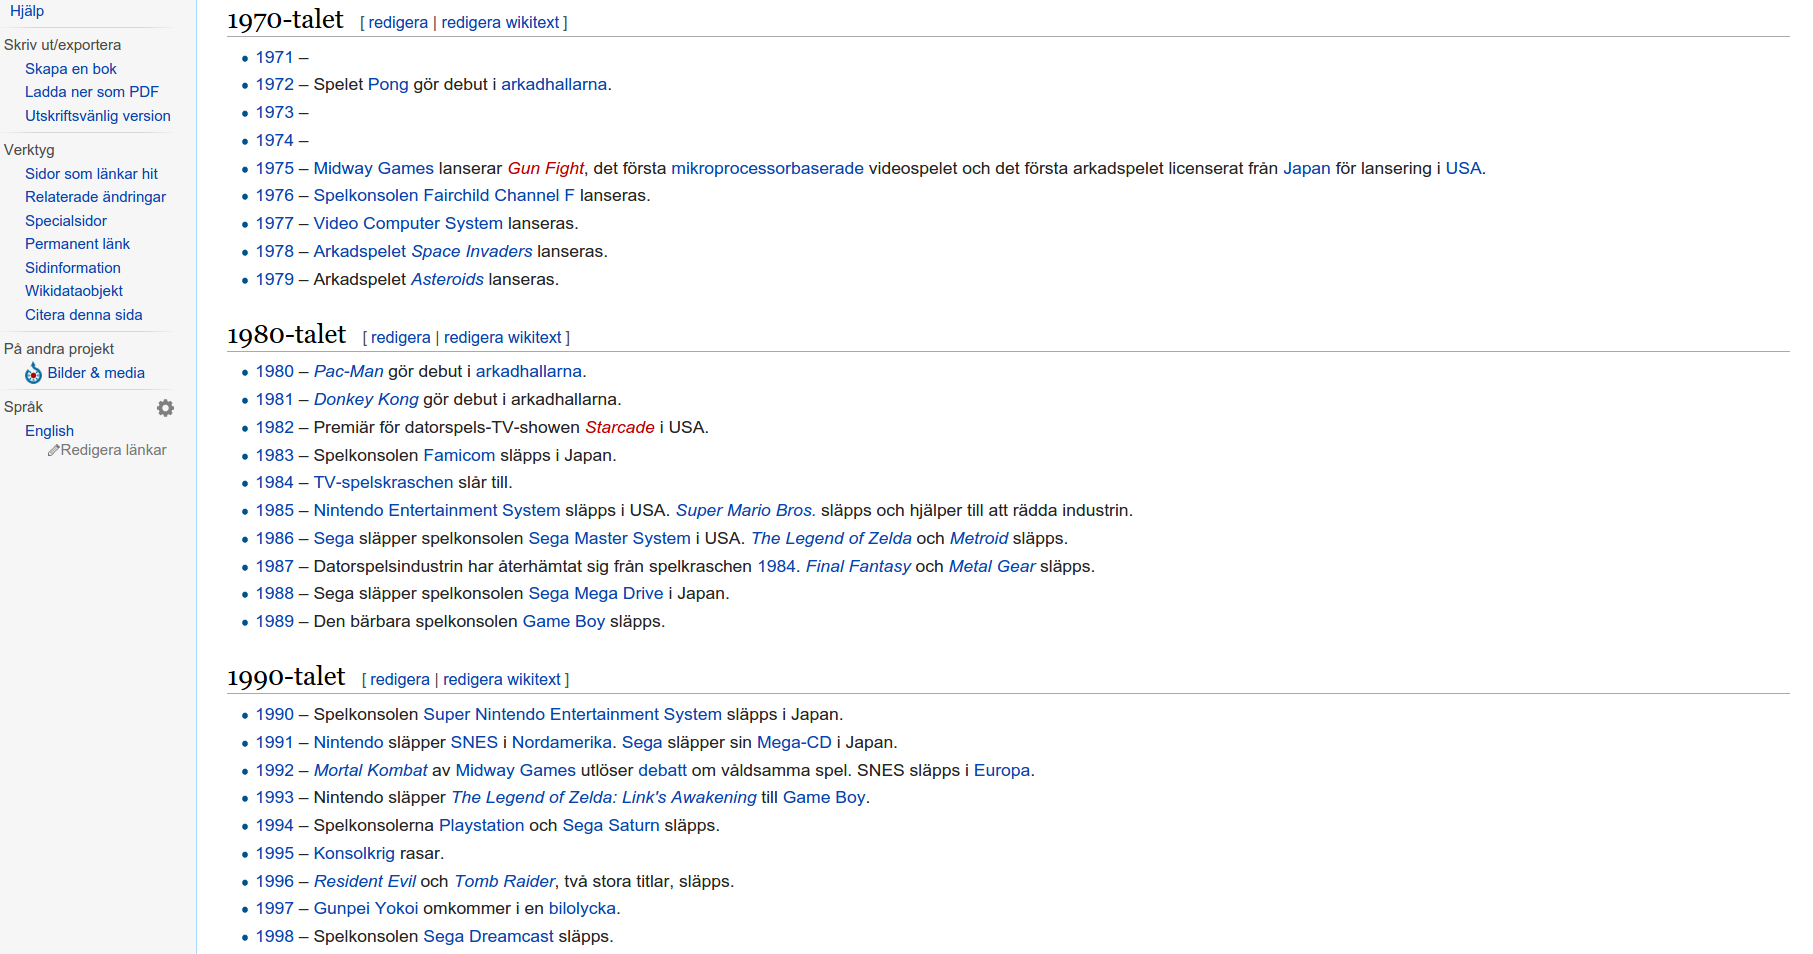
\includegraphics[width=\textwidth]{Listbild} 
	\end{centering}
	\caption{\textit{Ett exempel av listorna med årtal som Wikipedia tillhandahåller}}
\end{figure}

När alla  händelser har lästs in i cachet presenteras de inlästa händelserna en i taget i ett webinterface. Webinterfacet visar ett årtal, en fråga samt fyra knappar. Knapparna anger svårighetsgraderna lätt, medel eller svår samt ett alternativ för att ta bort den aktuella frågan helt.

\begin{figure}[H]
	\begin{centering}
	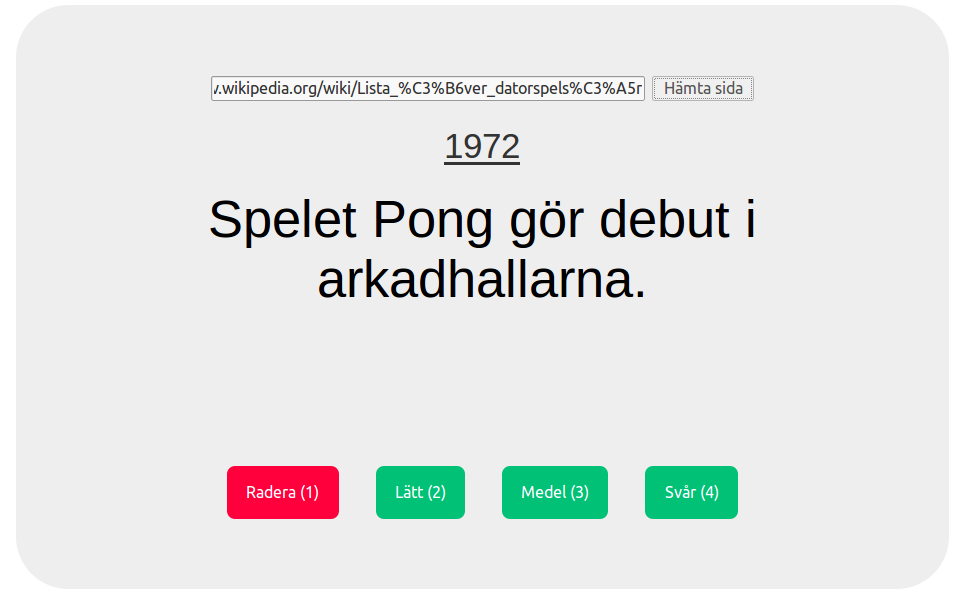
\includegraphics[width=\textwidth]{crawler} 
	\end{centering}
	\caption{\textit{Webinterface för crawlern}}
\end{figure}

De fyra knapparna är mappade till siffrorna 1-4 på tangentbordet för att det ska gå snabbt att gå igenom frågorna. Texten kan också redigeras om administratören vill justera grammatiska fel.

\subsubsection{Användare}
Det finns två sorters användare som kunde interagera med systemet.\\
\newline
\textbf{Administratörer} \label{admins}
Administratörerna är vi som utvecklade applikationen och som ansvarar för projektet. Vi är ansvariga för underhållet och utvecklingen av systemet. Vi har den högsta typen av tillgång till systemet för att kunna utföra underhållet och utvecklingen. I underhållet innefattas det felsökning samt reparation av funna fel. Underhållet innefattar även uppföljning av buggrapporter som skickats in av spelare. En vital uppgift som administratörerna har, förutom det allmänna underhållet och utvecklingen av systemet, är att godkänna information som hämtas av crawlern. Detta för att se till att frågorna följer den struktur som är lämplig för spelet.\\
\newline
\textbf{Spelare}\\
Spelarna är den typ av användare som har begränsad åtkomst till systemet. Spelarna kan endast komma åt systemet genom klienten och kan endast interagera med själva spelet. Detta innebär att en vanlig spelare inte ska kunna finna information om hur systemet fungerar. Detta är delvis en säkerhetsåtgärd som är till för att den vanliga användaren inte, av misstag, eller med flit ska kunna komma åt systemets vitala delar och alternera dessa. Användaren kan kommunicera med administratörerna genom att skicka felrapporter om spelet skulle bete sig konstigt eller om några buggar har upptäckts.

\subsubsection{Balanseringssystemet} \label{balanseringssystemet}
Balanseringssystemet hade två mål, dels att justera svårighetsgraden på frågorna som fanns i databasen och dels till att justera spelarnas svårighetsgrad. 

Det finns alltså två separata nivåsystem i applikationen. Varje fråga i databasen har ett siffervärde för dess svårighetsgrad, ju högre siffra, desto svårare fråga. På liknande vis hade också varje användare en svårighetsgrad som lagrats som ett siffervärde i spelarens profil. Syftet med dessa poäng är att få spelet att sätta upp så rättvisa och roliga matcher som möjligt för spelarna. 

\paragraph{Balansering av frågorna}

Frågornas svårighetsgrad justeras beroende på hur spelarna i matchen svarade på frågan. En fråga som det ofta svaras fel på ökar i svårighetsnivå allt eftersom fler spelare svarar fel. Svårighetsgraden är helt bunden till frågan i sig och finns alltså kvar mellan matcherna.

En frågas svårighetsgrad har ingenting med någon form av poängräkning att göra. Svårighetsgraden på frågorna finns till för att vid en matchstart kunna jämföras mot spelarnas svårighetsnivå. Med hjälp av detta kan spelet avgöra om frågan ska skickas till spelarna eller inte. Det handlar alltså helt och hållet om att spelet ska presentera frågor som är lagom svåra för spelarna, så att spelet ska bli lagom utmanande och maximalt roligt.

Om en spelare med låg nivå svarar rätt på en fråga så justeras frågans svårighetsgrad neråt. Ju högre nivå frågan har, desto större blir nedjusteringen. En spelare med hög nivå påverkar inte frågorna lika mycket som en spelare med låg nivå. Det här beror på att om en spelare med låg nivå svarar rätt på en svår fråga så var nivån på frågan förmodligen mycket mer felaktig än om en avancerad spelare svarat rätt på samma fråga. 

\paragraph{Balansering av spelarna}

Spelarnas svårighetsgrader justeras också efter avslutad match. Den här balanseringen går i stora drag till så att den vinnande spelaren tar poäng av den förlorande spelaren. Om den vinnande spelaren redan ligger på en högre nivå än den förlorande spelaren så tar hen väldigt lite poäng från förloraren. I det motsatta fallet tar istället den vinnande spelaren mycket poäng från den förlorande. Hur mycket poäng som faktiskt tas baseras på skillnaden i nivå mellan spelarna. 

Inspirationen till den här sortens balansering kom bland annat från Counter-strike: GO~\cite{cs} som använder sig av balanseringssystemet Elo~\cite{elo}. 

Balanseringen i Chronos ansågs vara tillräckligt bra med Elo för att användningen av ett mer avancerat system som Glicko skulle uteslutas. Det är också förmodligen så att ett spel som schack eller Counter Strike behöver mer frekvent träning för att spelare ska kunna behålla sin nivå än ett frågesportspel som Chronos. Allmänkunskap och historiekunskap är någonting som lättare förbättras i vardagen, än till exempel schacktaktik. 

I Chronos inträffar balanseringen efter en avslutad match. När hela matchen är avslutad finns alla frågor från matchen samt respektive spelares svar i serverns cache. Efter att en vinnare har utsetts anropas balanseringssystemet och både frågenivåerna och spelarnivåerna justeras utifrån matchens resultat.

\begin{verbatim}
downDiff = int((1.0-(userRatio*questionRatio))*10.0)
\end{verbatim}

Kodsnutten ovan är ett exempel på en justering som sker om en spelare har svarat rätt på den aktuella frågan. userRatio är ett värde mellan 0-1 på spelarens nivå (0 är nybörjare, 1 är avancerad). questionratio är ett värde mellan 0-1 på frågans nivå. downDiff är det värde som frågans nivå sänks med (mellan 0-10). 

\pagebreak
\subsection{Applikationens design}

\subsubsection{Genomgång av applikationen}
%Gör en genomgång av hur applikationen fungerar med en massa bilder som även har förklaringar till sig.\\

\large \textup{1. Inloggningsvy}\\
Första gången en användare startar applikationen eller av någon anledning har blivit utloggad möts hen av inloggningsvyn. Det är en webbsida som tillhandahålls av Google App Engine. Den innehåller primärt två textfält och en knapp för att logga in. När användaren fyllt i sina inloggningsuppgifter och klickat på logga in så sköter Google allt som har med inloggningen att  göra. Vår server får sedan ett unikt id för användaren och om det är första gången hen loggar in så skapas en egen användarstruktur som sparas in i databasen.
När detta är klart eller om användaren redan var inloggad stängs aktiviteten ner och istället öppnas matchvyn(2) upp. 
\begin{figure}[H]
	\begin{centering}
	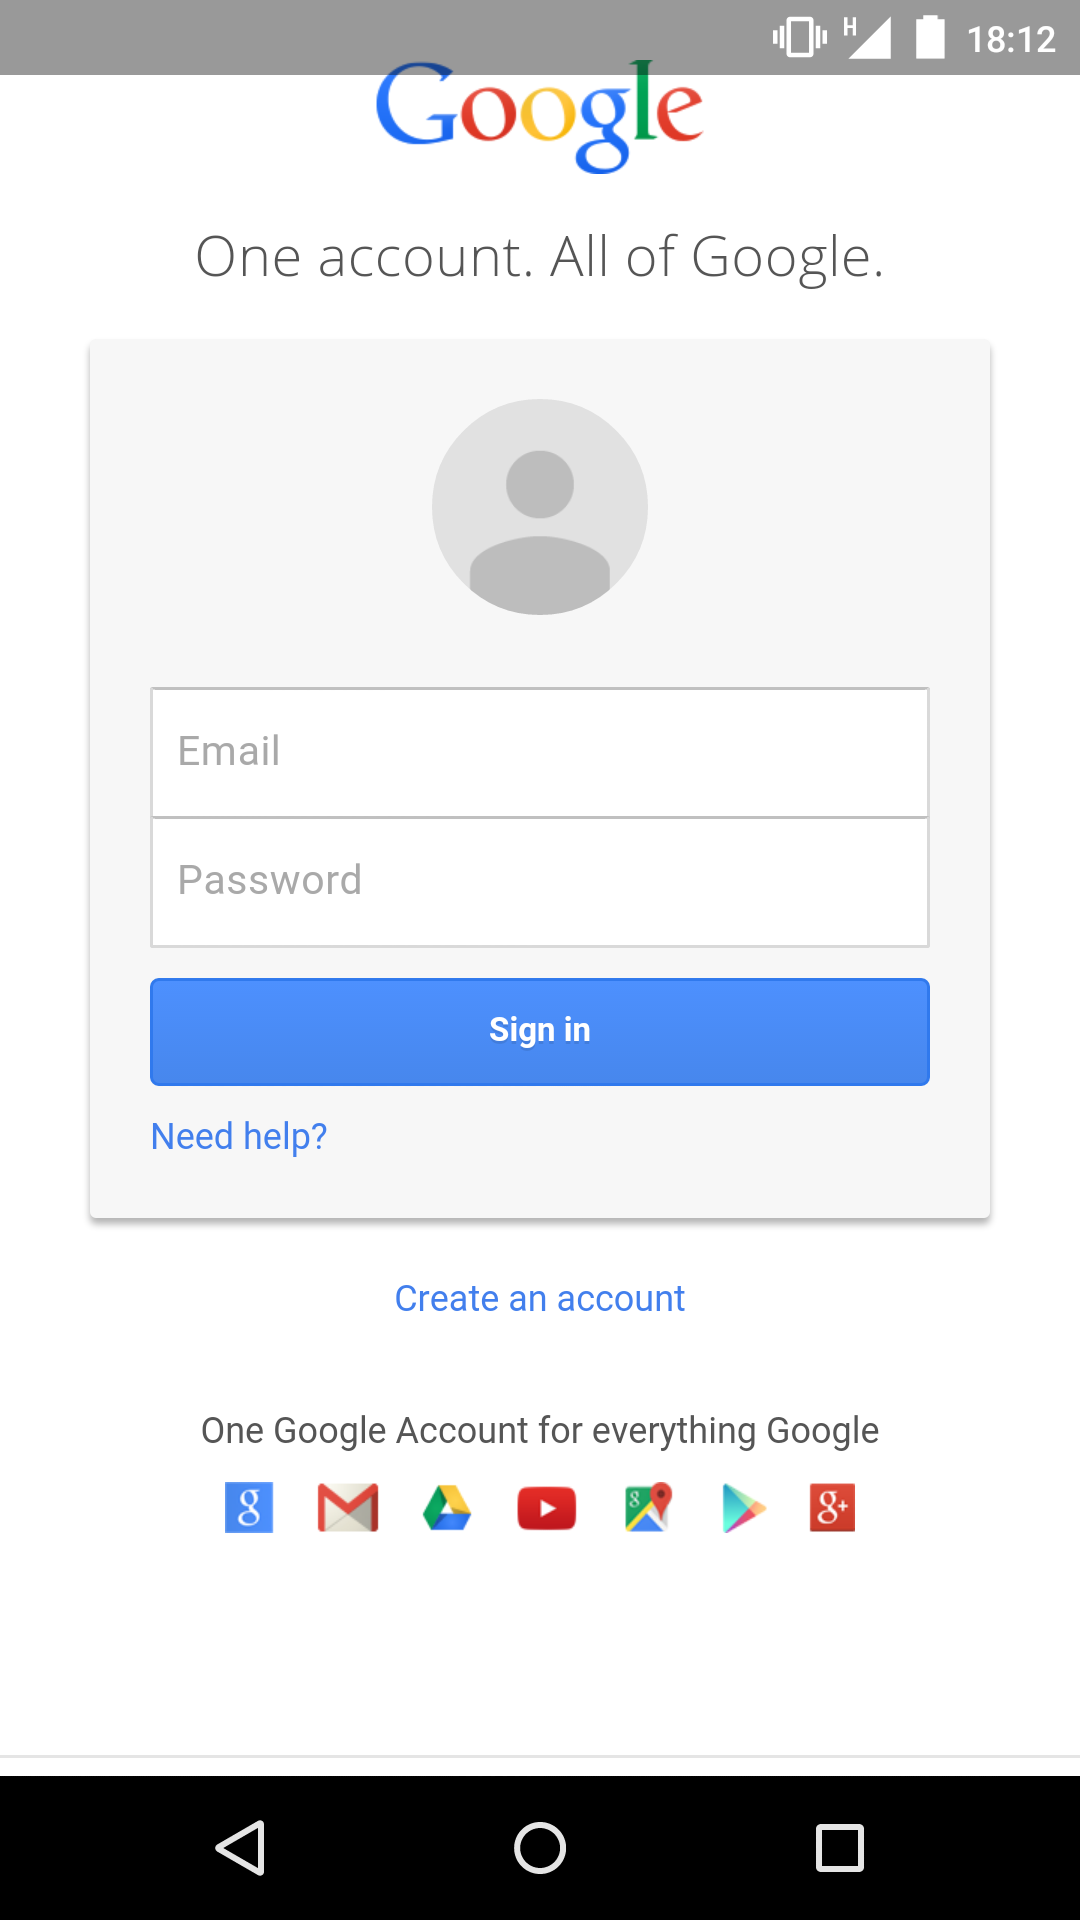
\includegraphics[width=0.4\textwidth]{app_login}\\ 
	\end{centering}
	\caption{\textit{Inloggningsvy}}
\end{figure}


\pagebreak
\large \textup{2. Startsida - Matcher}\\
Matchvyn kan lättast beskrivas som startsidan i hela applikationen. Det är här användaren ser vilka matcher hen har pågående eller har avslutat. I den här vyn kan användaren även starta en ny slumpad match samt söka efter en spelare eller vänner att utmana. 
Det finns fyra olika handlingar som användaren kan göra här vid denna sida. De kan klicka på hamburgarmenyn ($\equiv$) uppe i vänstra hörnet för att öppna navigationsvyn. De kan även klicka på en av de matcher de har pågående för att spela en ny omgång eller titta på matchens tillhörande matchstatistik. Om användaren väljer att klicka på en av matcherna skickas hen till matchstatistikvyn (3).
\begin{figure}[H]
\begin{center}
	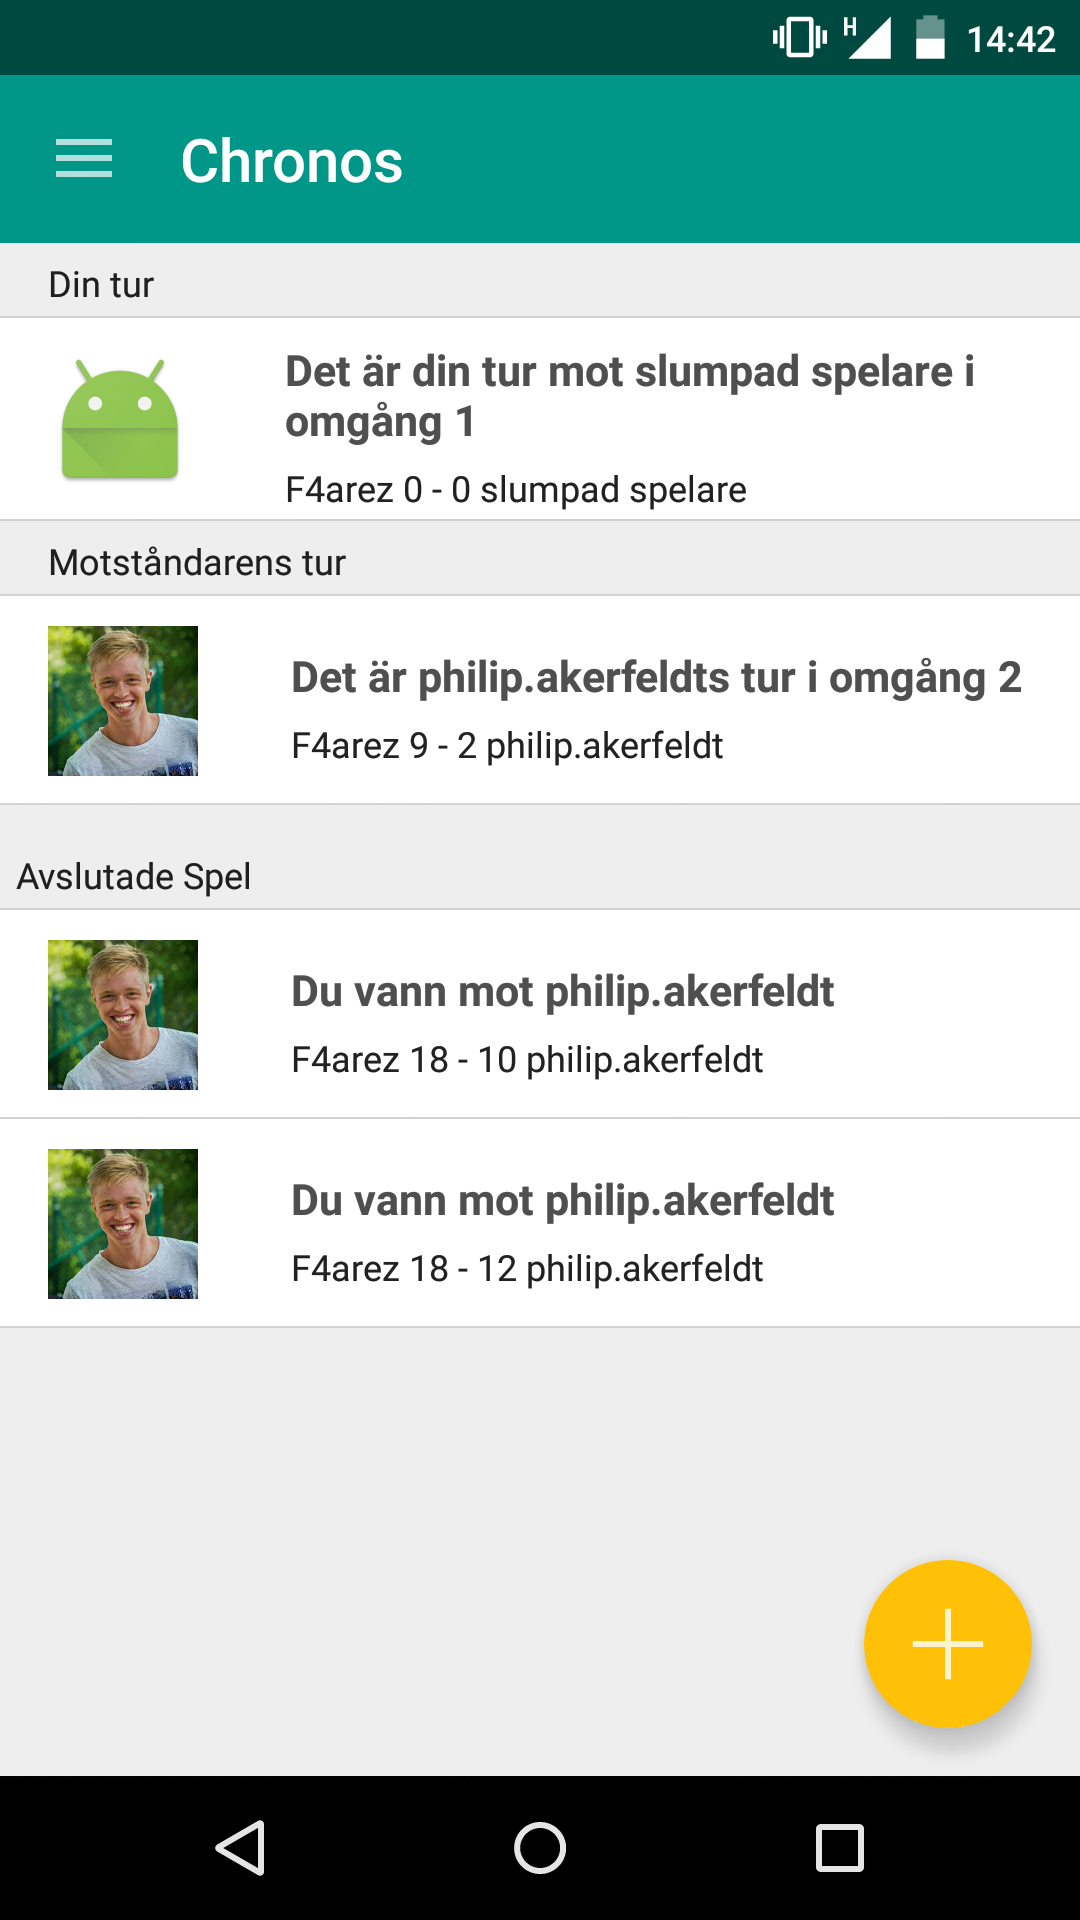
\includegraphics[width=0.4\textwidth]{app_matches} 
	\caption{\textit{Matchvyn - Startsidan i applikationen}}
	\end{center}
\end{figure}
\pagebreak

Användarna kan vid matchvyn dra med fingret neråt på skärmen för att uppdatera matchflödet. Detta är till för användaren ska kunna se om det blivit deras tur i en match eller om matchen är avgjord. Det finns även en så kallad \textit{Floating Action Button} (FAB). FAB är en del i Googles Material Design~\cite{MaterialDesign} och är en knapp som alltid ligger överst och representerar huvudhandlingen som kan göras på vyn. När FAB-en i denna vy klickas öppnas en dialog som ger användaren tre olika alternativ. De kan utmana en vän (Utmana en vän) när de klickar här byts vyn ut som ett rutnät av användarens vänner(7). 
De kan möta en slumpad motståndare (Slumpad motståndare) detta stänger ner dialogen som öppnades av FAB-en och en ny match finns i listan av matcher. De kan också söka efter en spelare(Sök spelare), då byts vyn ut mot en sökvy(8). 

\begin{figure}[H]
\begin{center}
	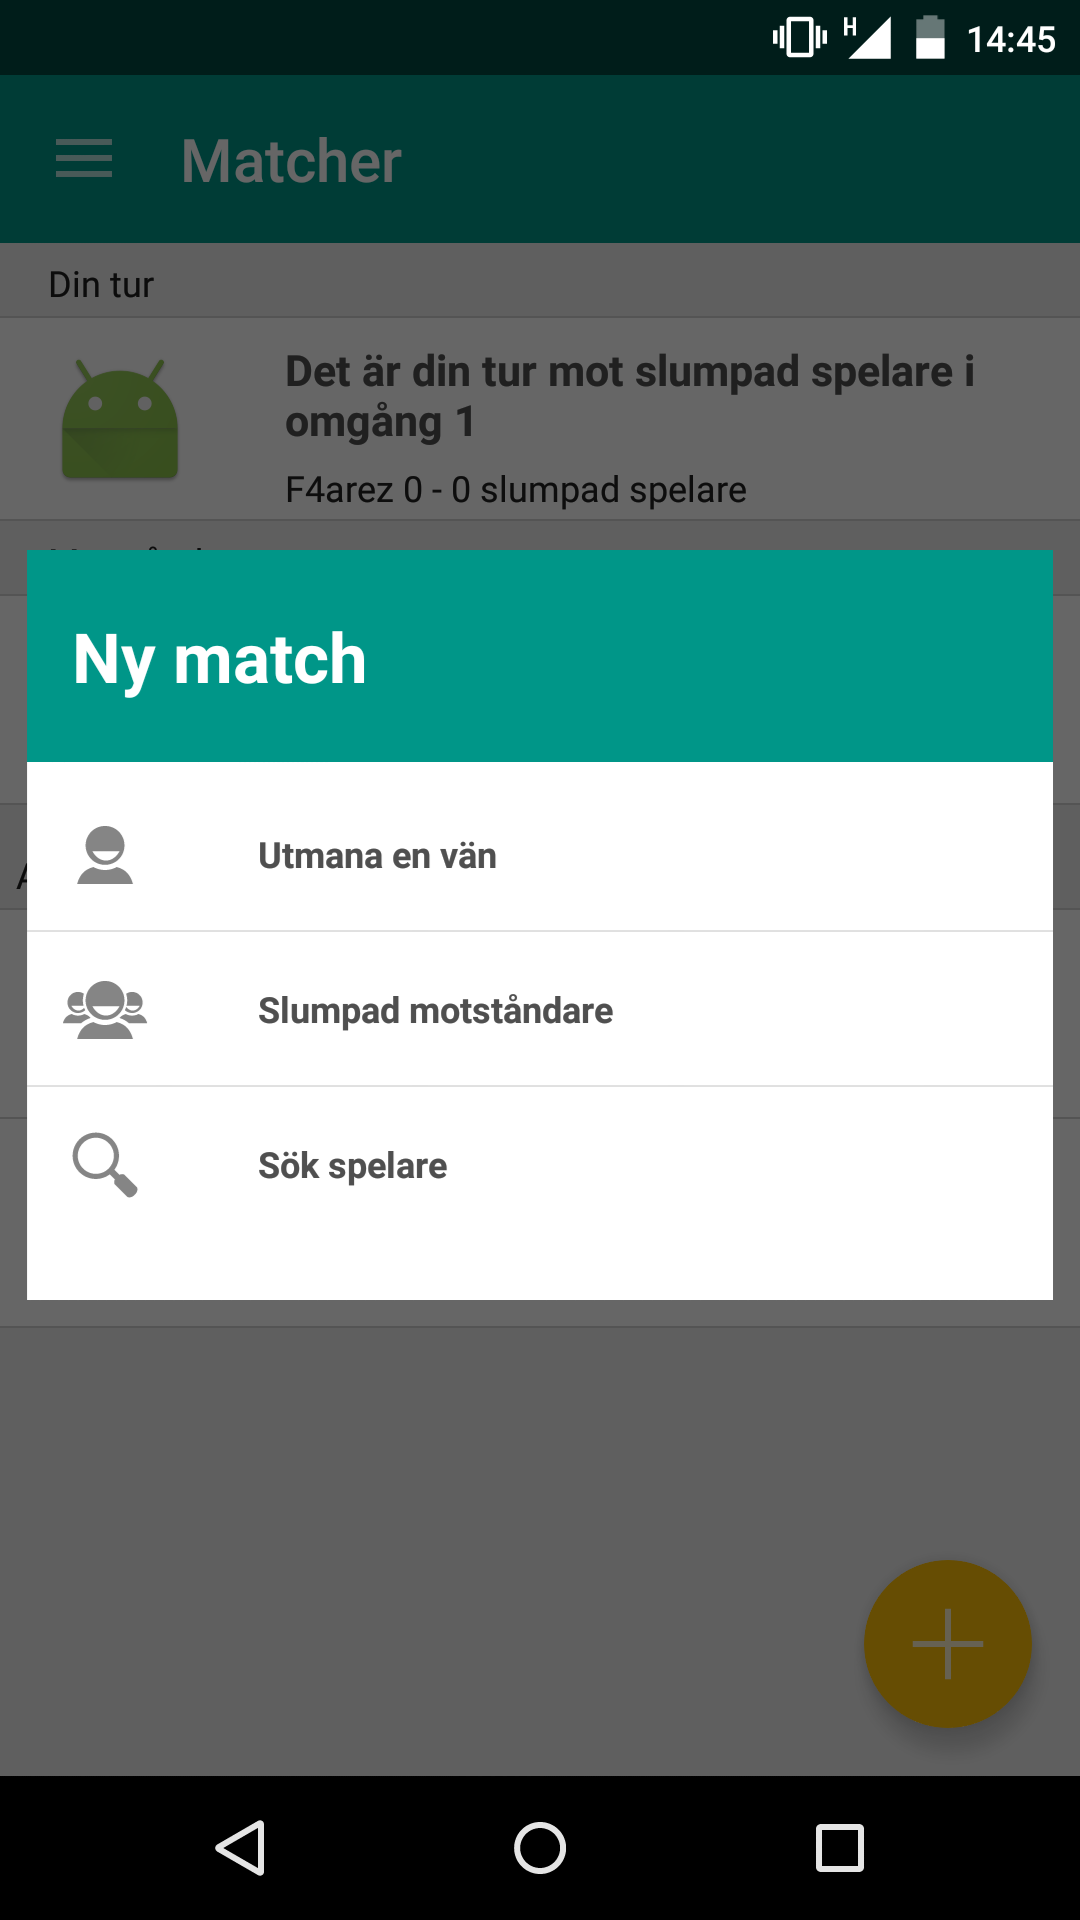
\includegraphics[width=0.4\textwidth]{app_new_match} 
	\caption{\textit{Dialogen som öppnas när man klickar på FAB-en}}
	\end{center}
\end{figure}

\pagebreak
\large \textup{3. Matchstatstik}\\
Hit kommer användaren när den klickar på en match eller när den har spelat färdigt en omgång. Vyn består av de två användarnas profilbild och namn och under det finns resultatet för varje runda som spelats. Längst ner finns två olika element, i mitten visas den sammanlagda poängen för hela matchen och till höger finns det en FAB som leder till en match(4)  


\begin{figure}[H]
	\begin{center}
	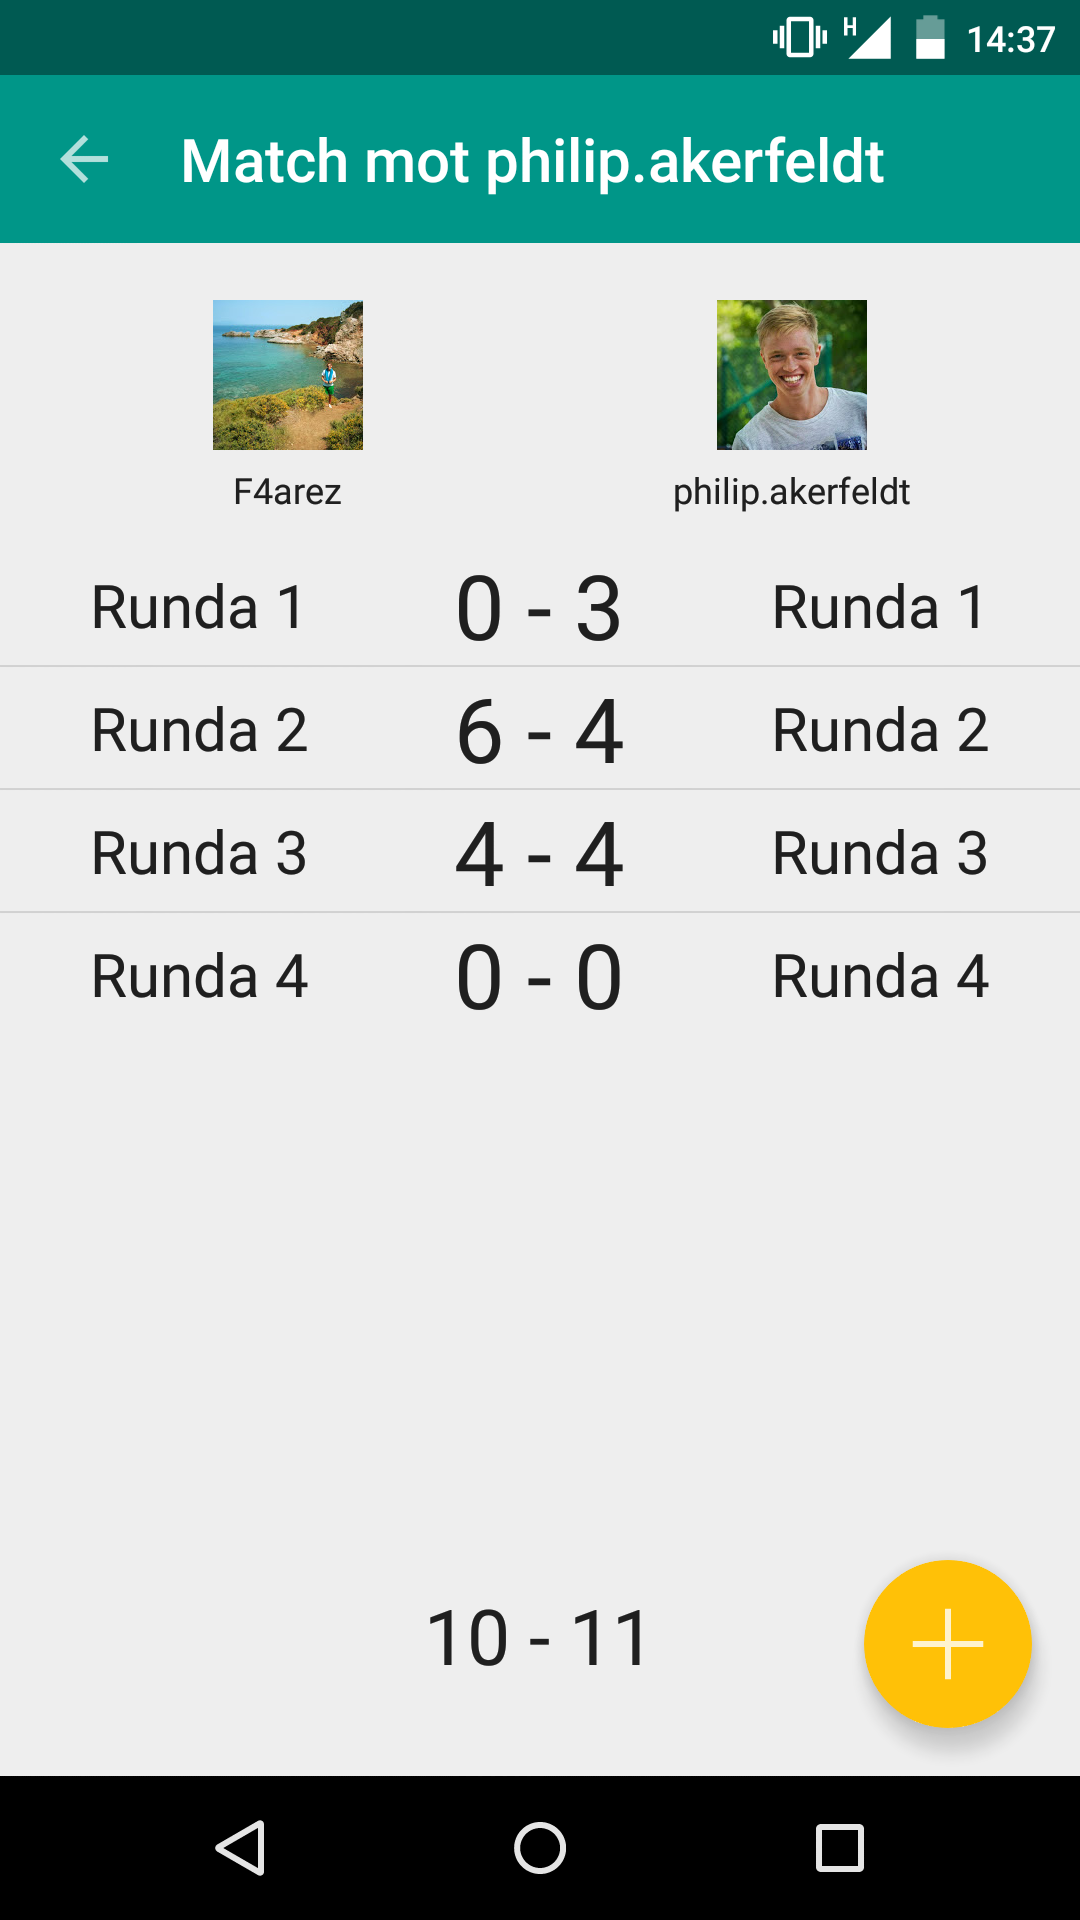
\includegraphics[width=0.4\textwidth]{app_match_stats} 
	\end{center}
	\caption{\textit{Vy över rundorna i en match}}
\end{figure}

\pagebreak
 \large \textup{4. Pågående match}\\
I figuren nedan illustreras hur spelet representerar en pågående match. Överst i vyn finns ett kort som innehåller den händelse som ska placeras in i tidslinjen. Under kortet ligger tidslinjen, den ska sorteras i kronologisk ordning där den tidigaste händelsen ligger högst upp. När matchen startas ligger det en given händelse i tidslinjen och ovanför ligger det en delare (Placera in händelsen i ordning). Delaren ska representerar händelsen som är skriven på kortet ovanför. Delaren är mobil och för att flytta den får man göra ett långt klick och sedan dra den den till den position man vill. Det finns även här en FAB som rättar placeringen av delaren, om svaret är rätt omvandlas delaren till händelsen som var på kortet och det läggs in en ny delare med en ny händelse som visas på kortet. Om svaret däremot var fel blinkar delaren till i rött och visar sedan årtalen på alla händelser som är utlagda i tidslinjen.


\begin{figure}[H]
	\begin{center}
	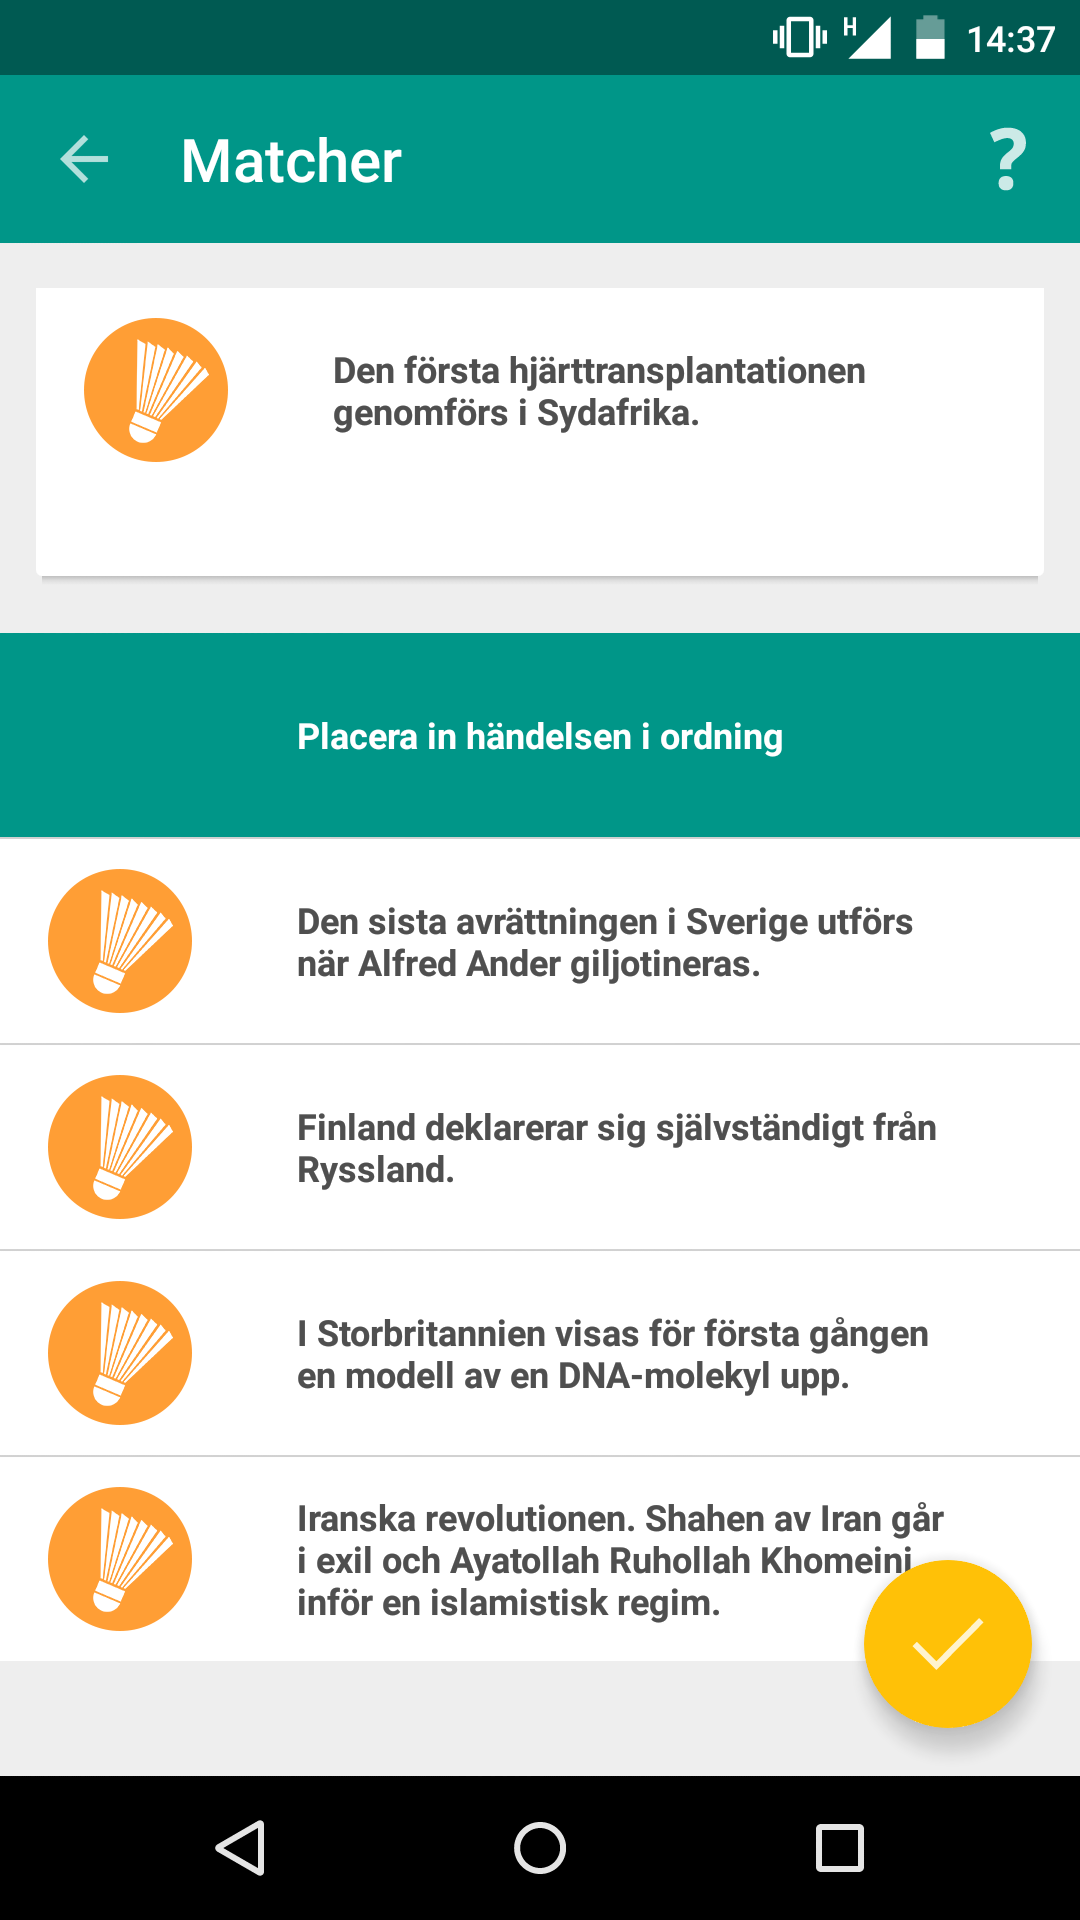
\includegraphics[width=0.4\textwidth]{app_match} 
	\end{center}
	\caption{\textit{Sceenshot på en match}}
\end{figure}



\pagebreak
\large \textup{5. Navigationsvy}\\
Navigationsvyn som illustreras nedan nås genom att klicka på hamburgarmenyn som finns i följande vyer: Startsida - matcher(2), Profilsida(6), Utmana en vän(7) och Sök spelare(8). Den ger möjlighet att navigera till de olika övermenyerna som finns: Startsida - Matcher (2), Inställningar (9), Min profil (10). Det finns även möjlighet att att köpa sig fri från annonser (Inga mer annonser) och att logga ut från sitt konto (LOGGA UT). Om spelaren väljer att logga ut skickas hen till inloggningsvyn(1). Högst upp i navigationsvyn finns det även en bild som fyller hela vidden av vyn. Bilden tas från användarens googlekonto och om hen inte har en omslagsbild visas istället en standardbild.   


\begin{figure}[H]
	\begin{center}
	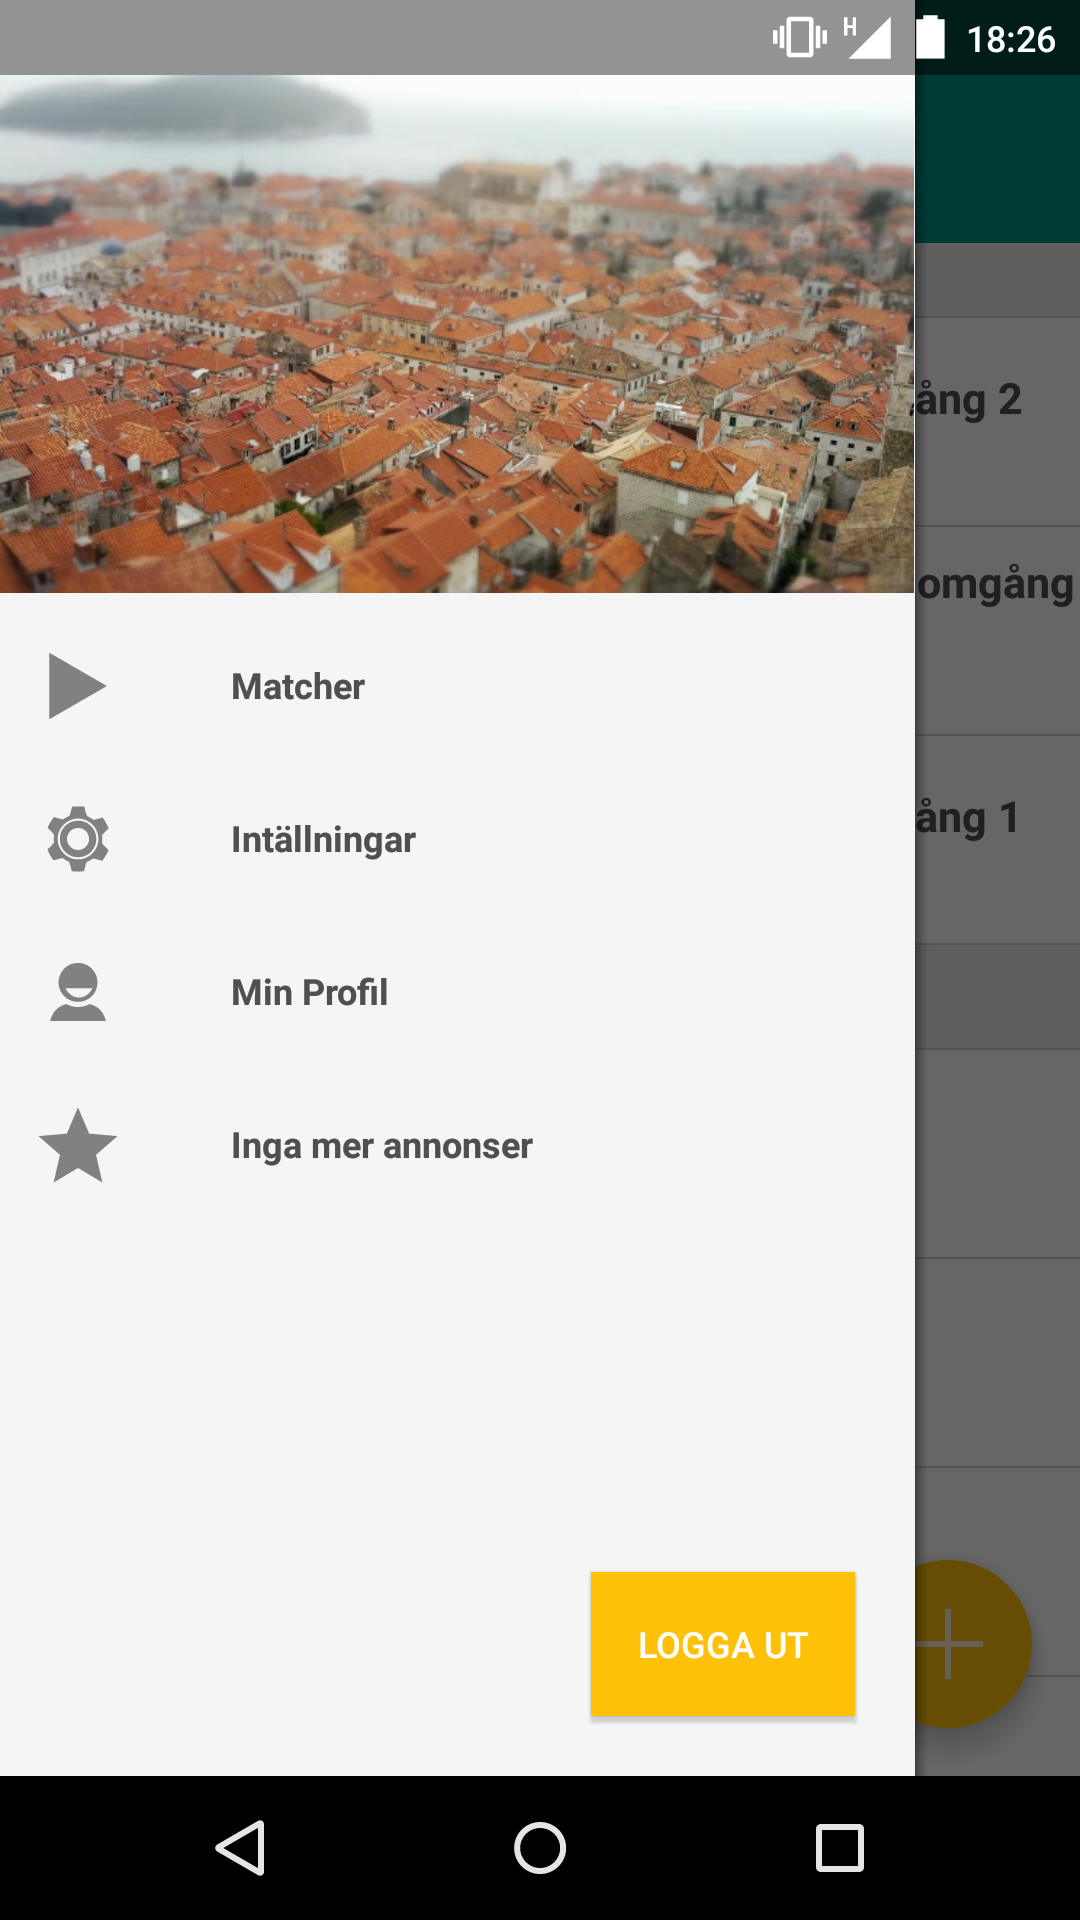
\includegraphics[width=0.4\textwidth]{app_drawer} 
	\end{center}
	\caption{\textit{Applikationens navigationsvy}}
\end{figure}


\pagebreak
\large \textup{6. Profilsida}\\
Det finns två sätt att komma till en profilsida. Man kan genom Min profil (10) klicka på en vän och få se deras profilsida eller genom Sök spelare (8). Vyn består av en profilbild som är tagen från användarens Googlekonto, längs kanten på profilbilden ligger det en FAB som vid tryck vecklas ut till ett verktygsfält där man kan utmana profilen (Utmana), lägga till profilen som en vän (Lägg till som vän) eller ta bort profilen från sin vän lista (Ta bort vän). Under profilbilden visas den andra användarens namn samt ett cirkeldiagram över hur många matcher som hen har vunnit, förlorat samt spelat oavgjort. Klickar man till exempel på den del som visar hur många matcher man förlorat visas det även hur många matcher det är man har förlorat. 




\begin{figure}[H]
	\begin{center}
	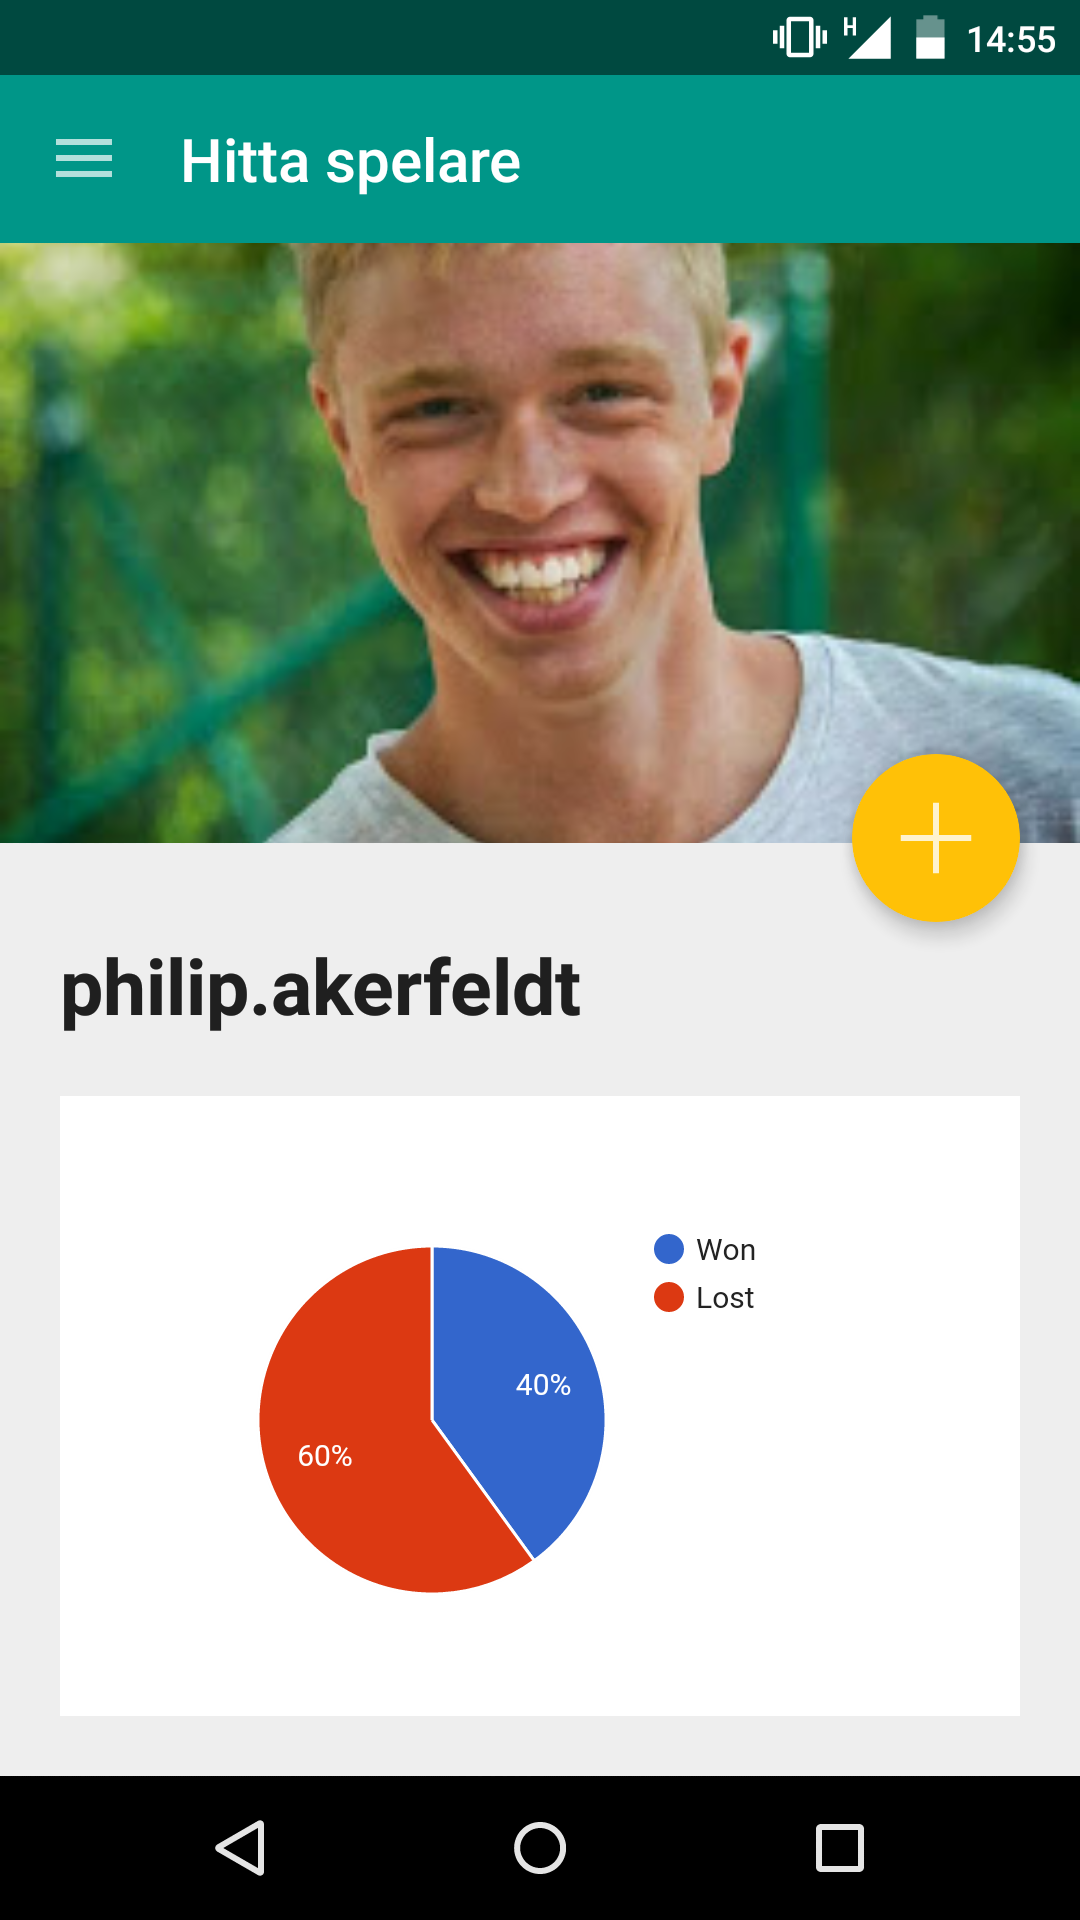
\includegraphics[width=0.4\textwidth]{app_profile_fab} 
	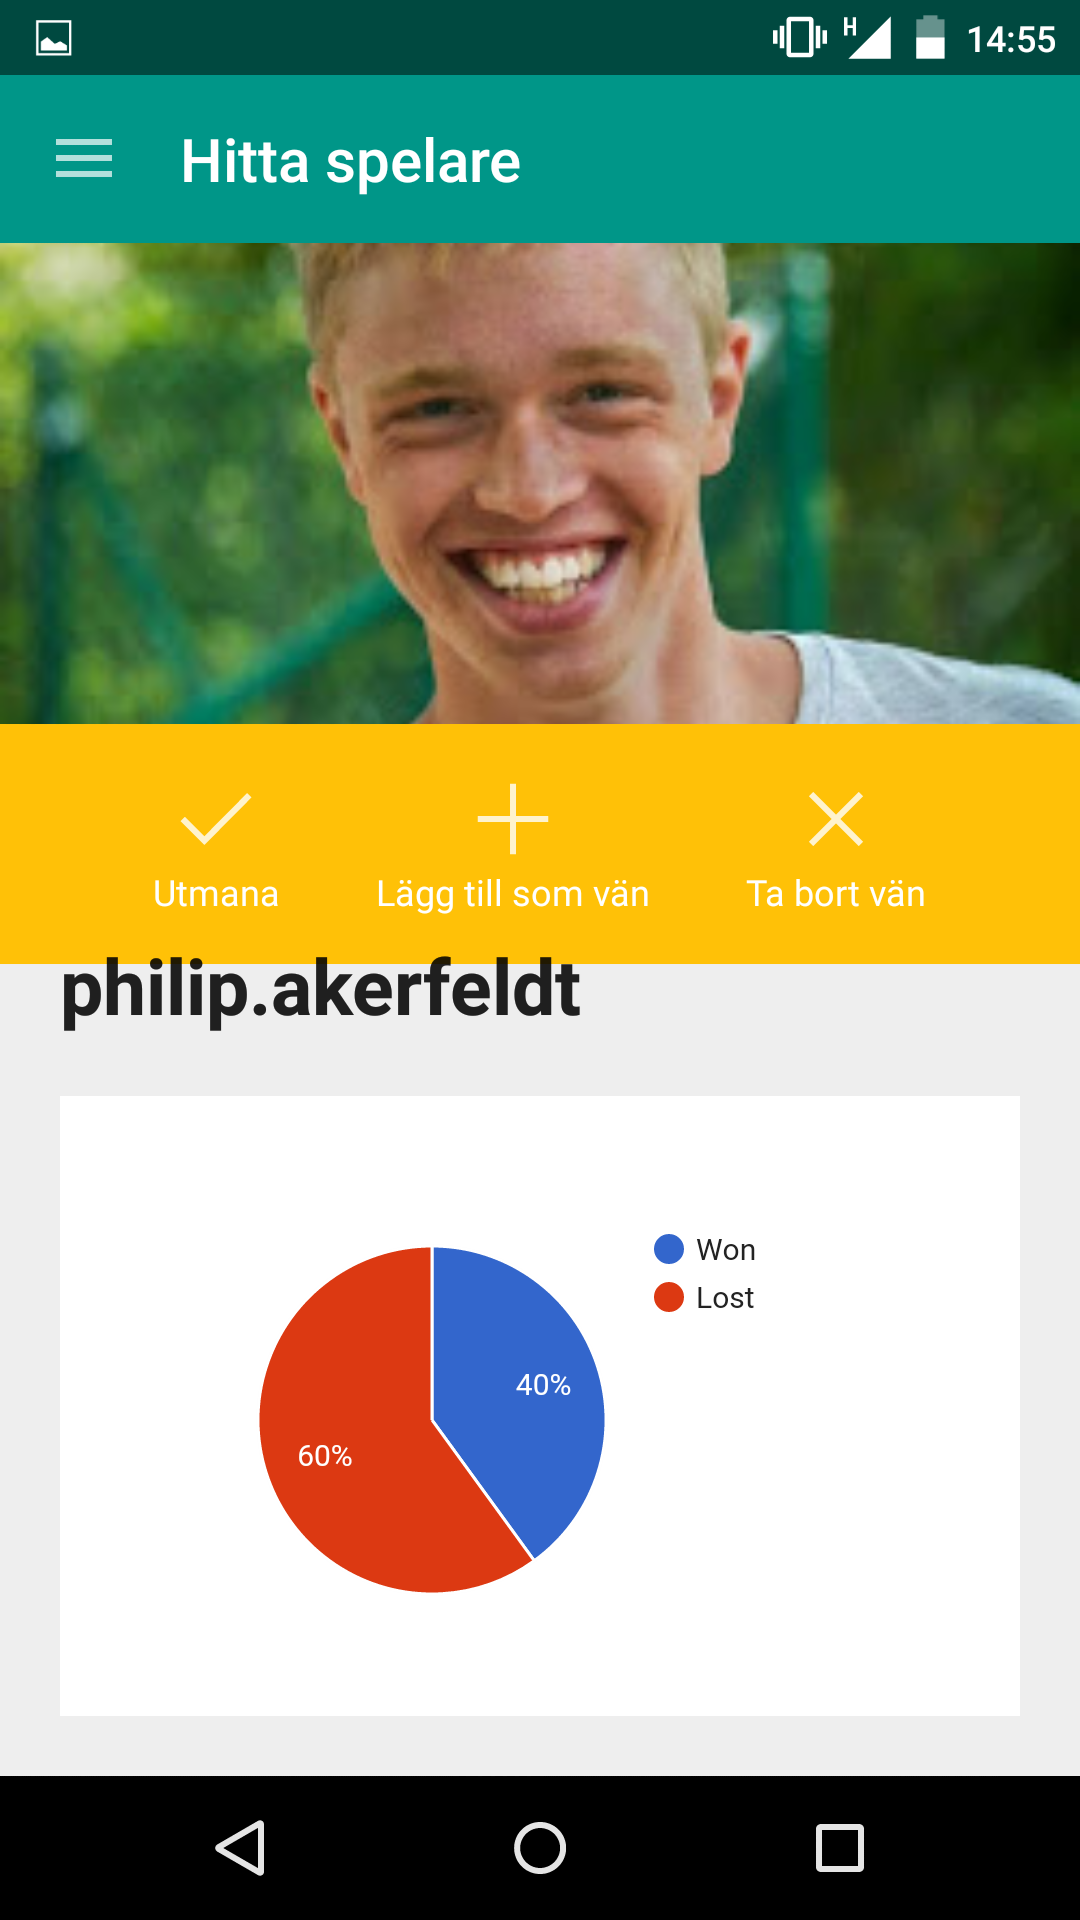
\includegraphics[width=0.4\textwidth]{app_profile_toolbar} 
	\end{center}
	\caption{\textit{Profilsida för en användare, till vänster med en FAB och till höger med ett verktygsfält som visas när användaren klickar på FAB-en }}
\end{figure}

\pagebreak
\large \textup{7. Utmana en vän}\\
Vyn består av ett rutnät av användarens vänner där varje väns profilbild och användarnamn syns. När användaren klickar på en vän skickas en utmaning till den vännen och det visas en Toast som säger att man utmanat vännen. 


\begin{figure}[H]
	\begin{center}
%	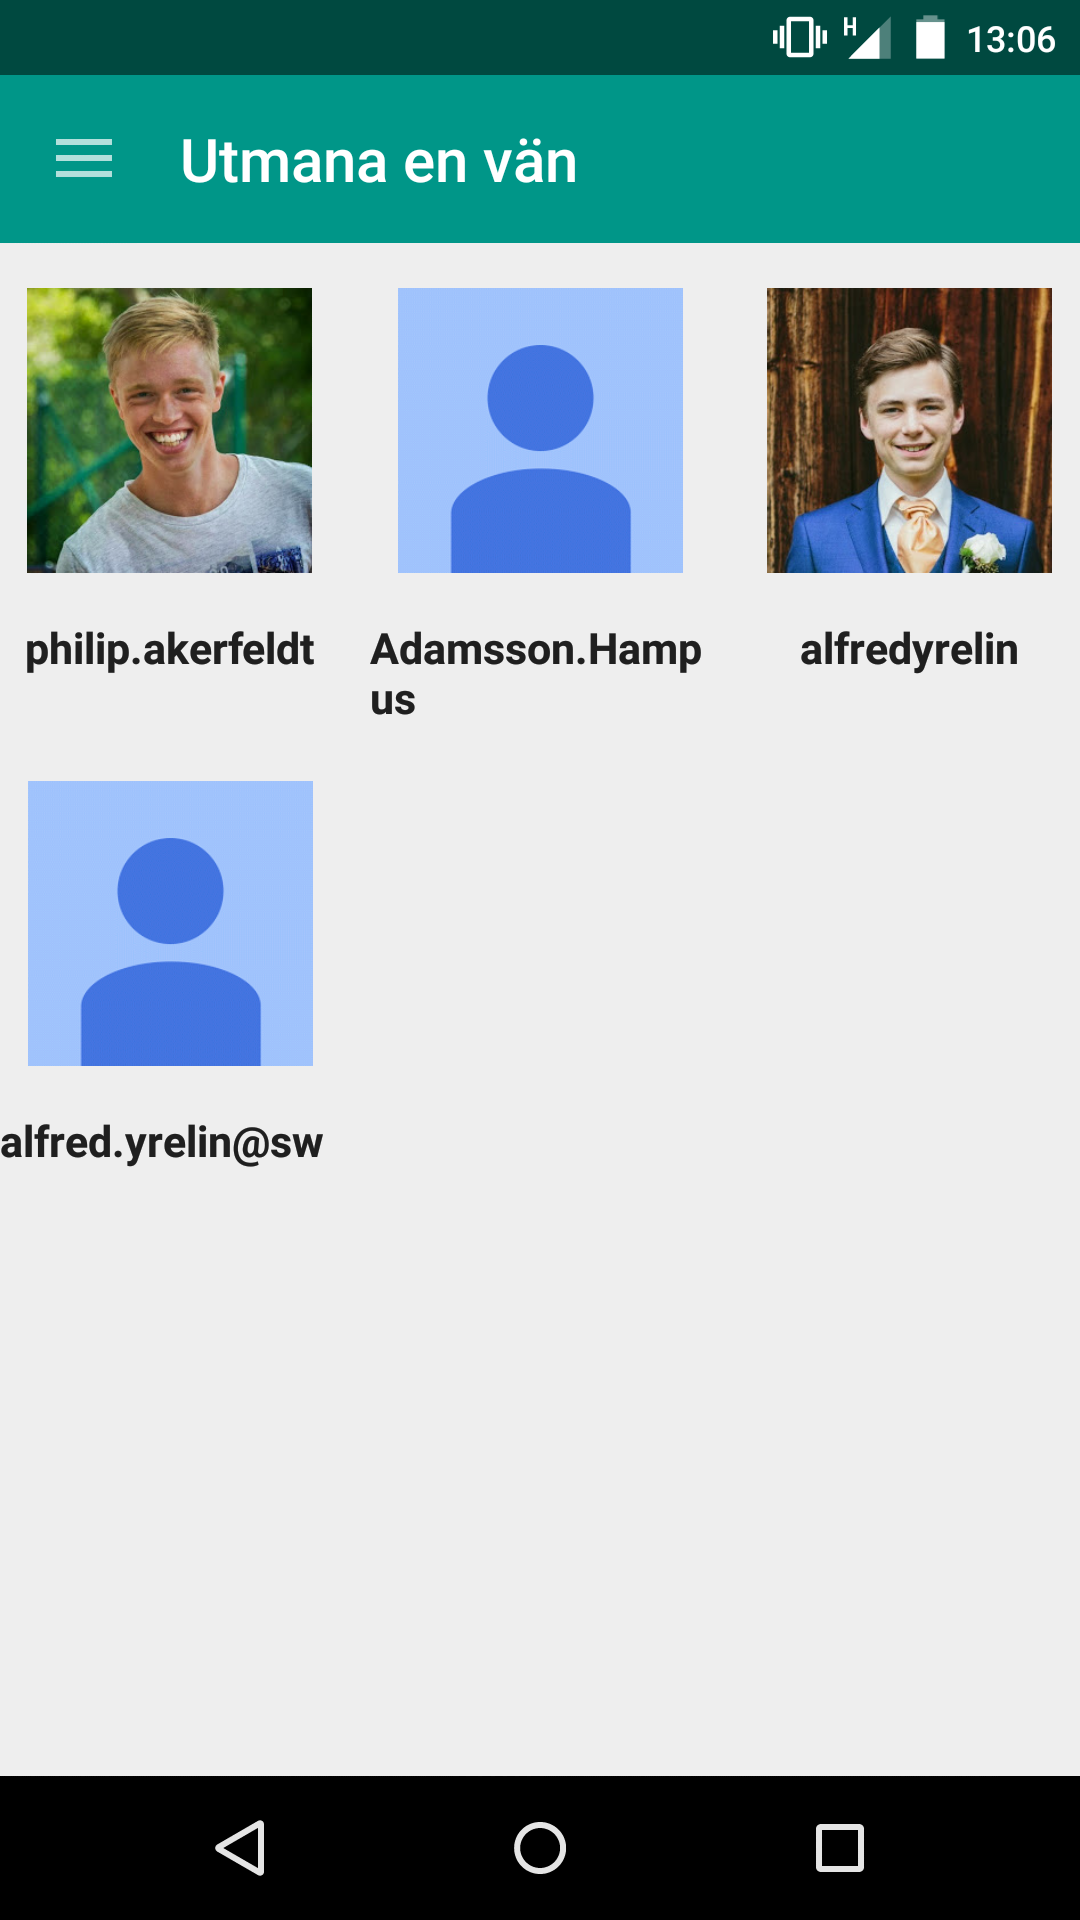
\includegraphics[width=0.4\textwidth]{app_challenge} 
	\end{center}
	\caption{\textit{Bild av vyn Utmana en vän(7)}}
\end{figure}

\pagebreak
\large \textup{8. Sök spelare}\\
När denna vy startas visas först bara söklinje upp, men när man sedan fyller i tecken och klickar retur visas ett rutnät av personer som matchar sökningen. Varje sökresultat visar profilbild och användarnamn. Klickar man på något av sökresultaten tas man till dennes profilsida(6)  
\begin{figure}[H]
	\begin{center}
%	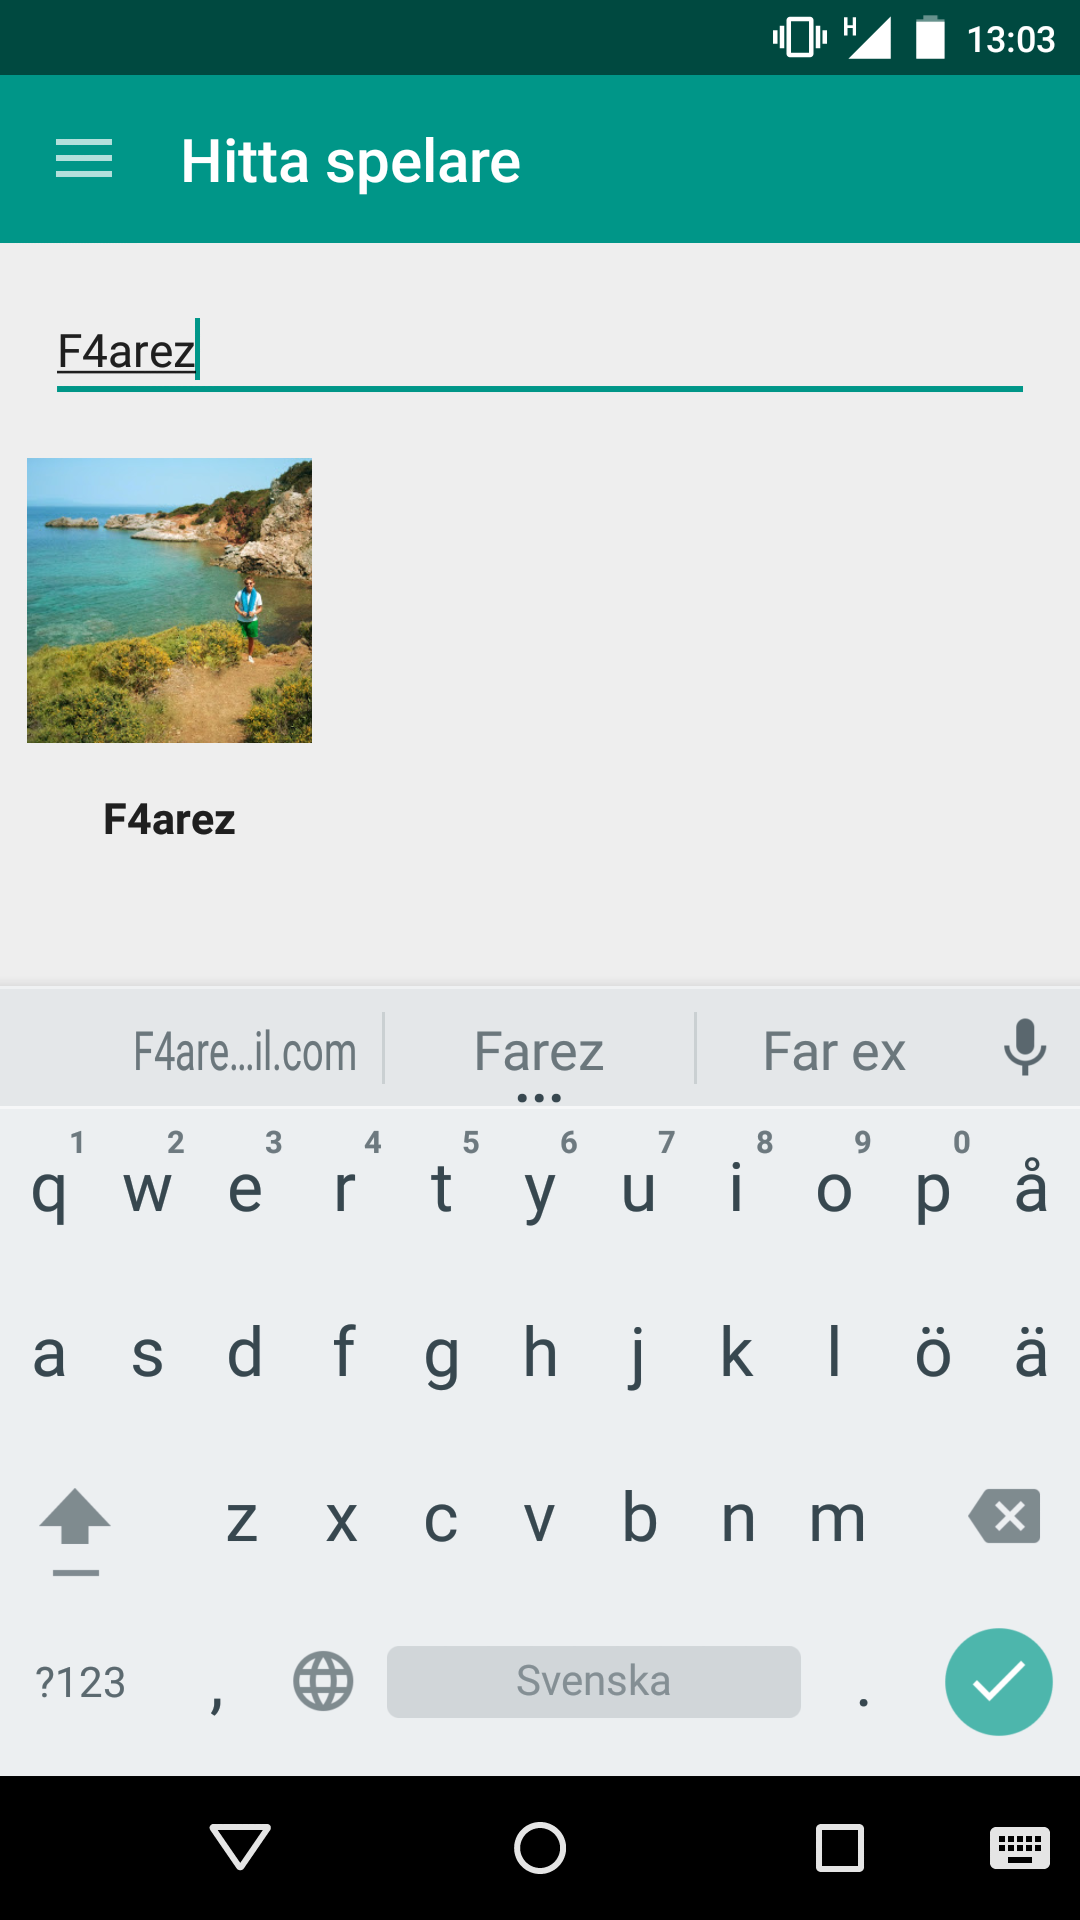
\includegraphics[width=0.4\textwidth]{app_search} 
	\end{center}
	\caption{\textit{Bild av vyn Sök spelare(8) när en användare hittats}}
\end{figure}



\pagebreak
\large \textup{9. Inställningar}\\

\pagebreak
\large \textup{10. Min profil}\\
Överst på vyn finns det ett cirkeldiagram som innehåller statistik över hur många matcher som vunnits, förlorats eller slutat oavgjort. Under finns ett rutnät av användarens vänner som visas med hjälp av deras profilbild och användarnamn, klickar man på en vän visas deras profilsida(6). 

\begin{figure}[H]
	\begin{center}
%	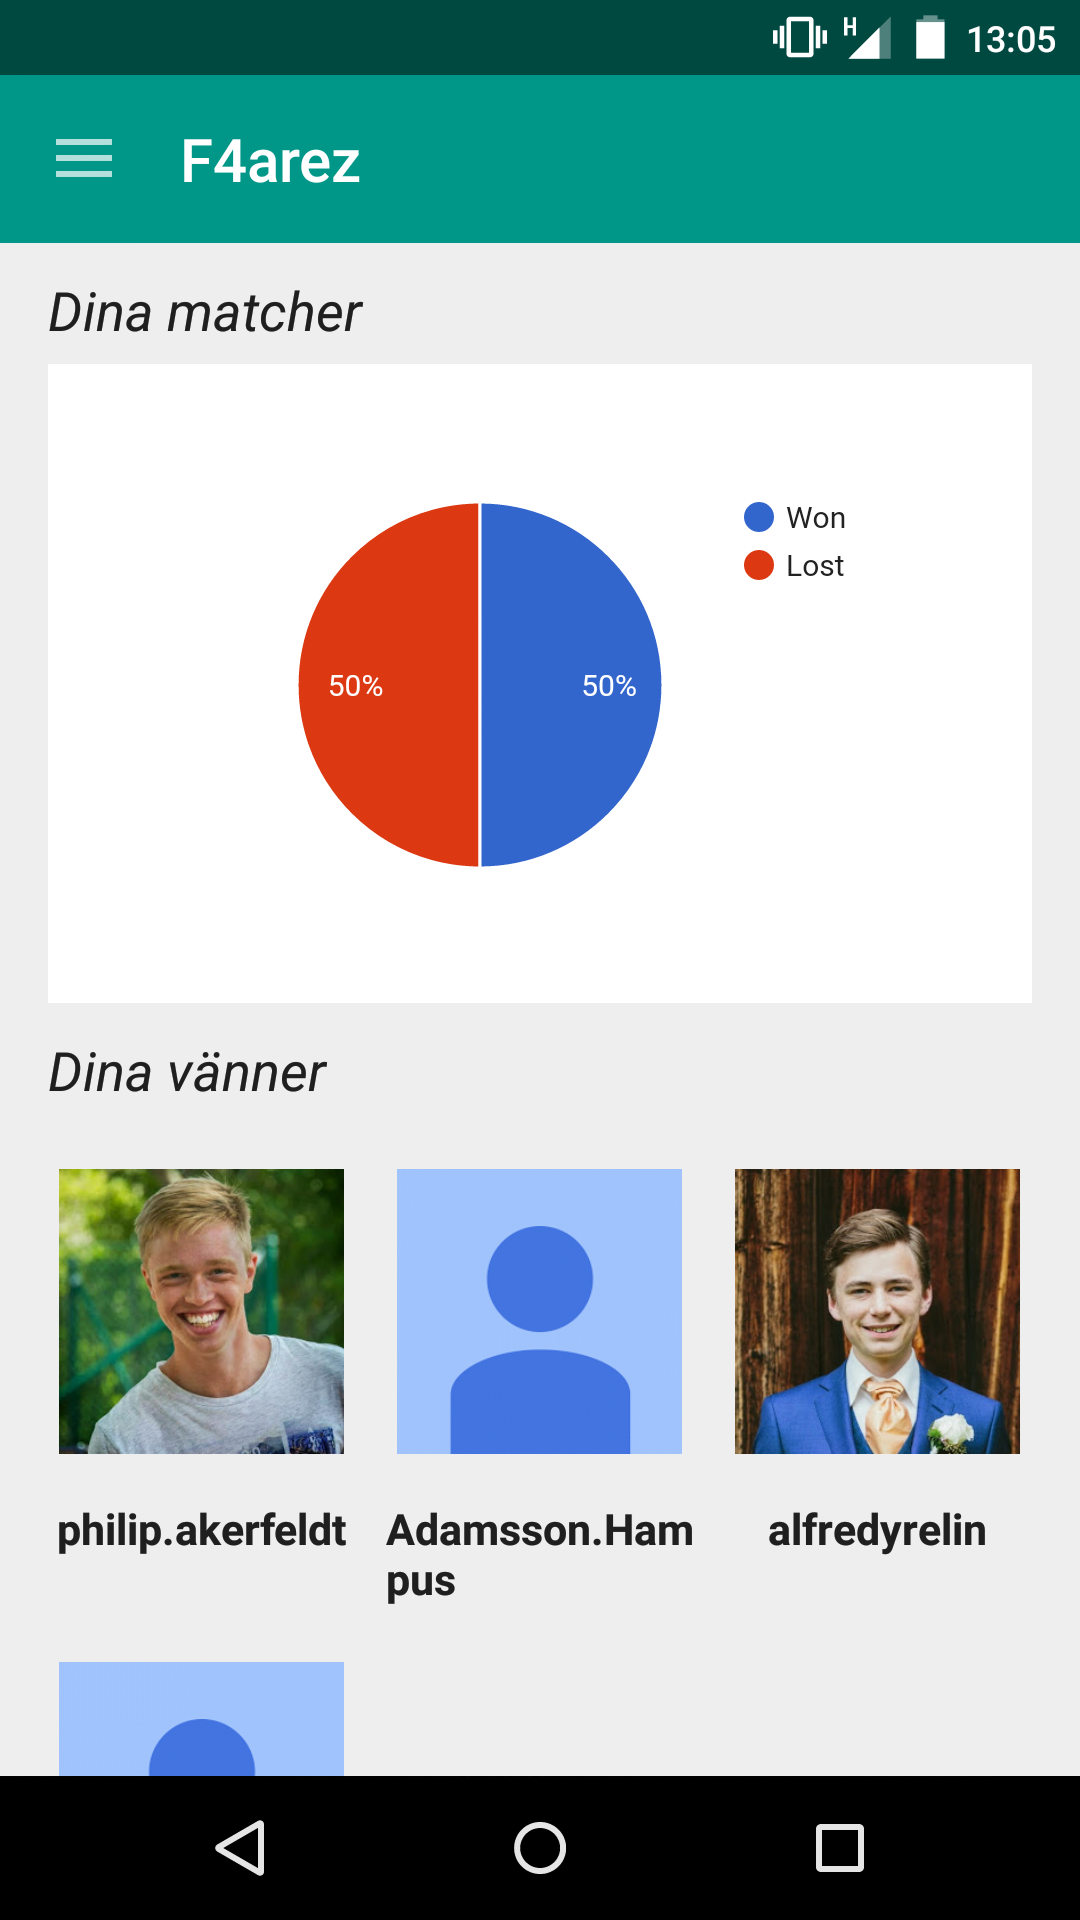
\includegraphics[width=0.4\textwidth]{app_profile} 
	\end{center}
	\caption{\textit{Bild över Min profil (10)}}
\end{figure}


\section{Resultat}
Den här sektionen beskriver de utvärderingar som gjorts av applikationen. Utvärderingarna gjordes bland annat för att fastställa applikations användarvänlighet men också för att få nödvändig feedback på applikationens utseende och effektivitet. Det utfördes tre utvärderingar på applikationen. En \textit{Think Aloud}, en \textit{Kognitiv Genomgång} och en \textit{Heuristic Evaluation}. 

\subsection{Utvärderingar och deras användbarhet}
Utvärderingar är bra verktyg för att hitta problem eller för att hitta områden som är lämpade för vidare utveckling. Det kan också hjälpa till att få nyttig feedback på en tidig design eller hjälpa till att välja mellan olika designalternativ~\cite[sid 226--228]{benyon2010designing}. Utvärderingarna vi valde att utföra var till för att granska produkten vi har utvecklat. Vi ville se om produkten mötte de krav som vi hade ställt vid starten av projektet. Vi hoppades även att utvärderingarna skulle ge oss en bild av applikationens användbarhet och effektivitet samt se till att den var tillmötesgående. Ur en designsynpunkt gjorde vi utvärderingen för att se om applikationen fyllde sitt syfte, om den var rolig samt om den engagerar användaren.


\subsection{Utvärdering av projekt}
Planen var att en fungerande alfa eller betaversion av systemet skulle färdigställas en rimlig tid innan projektet avslutas. I den här versionen skulle användare ha möjlighet att ge feedback och att testa applikationen. Tack vare den feedback vi fick från användarna så skulle så många fel som möjligt justeras innan den färdiga versionen släpptes.



\subsection{Kognitiv Genomgång}
En \textit{Kognitiv Genomgång}~\cite[sid 2--8]{cognitive} är en utvärderingsmetod som är till för att avgöra problem med användbarhet i ett interaktivt datorsystem. Utvärderingen går ut på att utvecklarna traverserar systemet analytiskt givet ett antal specifika uppgifter användarna förväntas utföra i systemet. Den kognitiva genomgången utvärderar vilken sekvens av steg som är nödvändiga för att användaren ska kunna utföra en uppgift. Användarnas sekvens av steg jämförs sedan med utvecklarnas förväntade sekvens för att utföra samma uppgift. Detta för att se skillnader i sekvenserna och därmed upptäcka problem med den aktuella designen.\\
Innan utvärderingen kan utföras måste utvecklarna göra en komplett lista med steg för att lyckas göra varje uppgift korrekt. Förutom detta behöver utvecklarna bestämma fyra faktorer:
\begin{enumerate}
\item Vilka kommer använda systemet?\\
Ett exempel på en fråga som är hjälpsam vid ett sådant val är exempelvis: "Vilken typ av bakgrundskunskap behöver användarna för att kunna använda systemet?"
\item Vilka uppgifter i systemet ska analyseras?
\item Vilken är den rätta ordning av handlingar för att utföra uppgiften?
\item Definiera gränssnittet.
\end{enumerate}

När detta är fastställt kan utvecklarna börja med utvärderingen. Under utvärderingens gång ska utvecklarna ställa följande frågor vid varje vald uppgift. Kommer användarna försöka uppnå rätt mål? Kommer användarna märka att rätt beslut är tillgängligt? Kommer användaren kunna koppla rätt beslut till det målet hen försöker uppnå? Om rätt beslut har tagits, kommer användaren förstå att hen har gjort framsteg i att uppnå målet?
Om någon av dessa frågor får ett negativt svar betyder det att det finns problem i användbarheten och detta noteras då av utvecklarna~\cite[sid 230--232]{benyon2010designing}.\\

Efter utvärderingen kan utvecklarna analysera den data som samlats in och skapa en ny design eller alternera den gamla för att öka användbarheten.\\ 

En stor fördel som gjorde att vi valde att använda oss av en kognitiv genomgång är bland annat metodens välstrukturerade process. Bortsett från detta är en av metodens stora styrkor att den bygger på en väletablerad teori till skillnad från många andra metoder som är av typen \textit{trial and error}~\cite[sid 230-231]{benyon2010designing}.\\

\subsubsection{Förberedelse inför kognitiv genomgång av Chronos} \label{kog}
Den typen av användare som vi valde att utveckla Chronos för är en person som har en smartphone med operativsystemet Android 4.4 eller senare. Det krävs även av användaren att hen har ett konto hos Google, exempelvis ett gmail-konto. Kunskapsmässigt krävs det att användaren vet hur en smartphone används samt besitter kunskaper om hur applikationer fungerar. Utöver detta krävs inget för att kunna använda sig effektivt av Chronos.
De uppgifter som användaren hoppas genomföra är att starta upp applikationen och logga in med sitt Google konto. Starta en match mot en slumpad motståndare och spela klart den slumpade matchen. Söka och lägga till en vän samt utmana den tillagda vännen och spela klart matchen samt till sist logga ut ur applikationen.\\
Den korrekta sekvensen av handlingar för att genomföra dessa uppgifter är:
\begin{enumerate}
\item Starta applikationen.
\item Logga in med Googlekonto.
\item Skapa en ny match mot slumpad motståndare genom att trycka på \textbf{+}-ikonen längst nere i vänstra hörnet och välja alternativet \textit{Slumpad motståndare}.
\item Välj den slumpade matchen genom att klicka på listelementet som ligger under rubriken \textit{Din tur}. 
\item Starta rundan genom att trycka på \textbf{+}-ikonen.
\item Vid avslutad runda används telefonens bakåtknapp, alternativt Chronos knapp \textbf{"$\leftarrow$ Matcher"}, för att gå tillbaka till matchsidan.
\item Repetera steg 5 \& 6 tills dess att matchen är avslutad.
\item Sök efter en vän genom att trycka på \textbf{+}-ikonen längst nere i vänstra hörnet och välja alternativet \textit{Sök spelare}.
\item Skriv in spelarens namn.
\item Välj önskad användare genom att klicka på användarens bild.
\item Tryck på \textbf{+}-ikonen vid användarens bild för att lägga till som vän.
\item Tryck på \textbf{+}-ikonen vid användarens bild för att utmana vännen.
\item Repetera steg 5 \& 6 till dessa att matchen är avslutad.
\item För att logga ut från applikationen tryck på knappen \textbf{$\equiv$} och välj sedan alternativet \textbf{Logga ut} längst ner i menyn.
\end{enumerate}

Miljön som utvärderingen utförs i är applikationen Chronos på en smartphone med operativsystem Android 4.4 eller högre.

\subsubsection{Simulering av kognitiv genomgång av Chronos}
Detta är en simulerad körning av applikationen med användaren, uppgifterna och miljön som är beskrivna i \ref{kog}.\\
\begin{enumerate}
\item Starta applikationen. \\ 
Detta är något som en person som äger en smartphone kommer kunna utföra genom kunskap från erfarenhet.
\item Logga in med Google konto.\\ 
Om användaren har ett konto hos Google så kommer det inte uppstå några problem här då hen tidigare har tvingats logga på andra platser med liknande layout.
\item Skapa en ny match mot slumpad motståndare genom att trycka på den gröna cirkulära \textbf{+}-ikonen längst nere i vänstra hörnet och välja alternativet \textit{Slumpad motståndare}.\\
Vid denna punkt presenteras användaren med en vy som är blank förutom den gröna cirkulära \textbf{+}-ikonen. Tack vare att användaren är van vid att använda sig av applikationer kommer hen trycka på den gröna cirkulära \textbf{+}-ikonen.
\item Välj den slumpade matchen genom att klicka på listelementet som ligger under rubriken \textit{Din tur}.\\
Vyn som användaren ser framför sig nu är tom med undantaget för en match som beskriver att det är spelarens tur mot en slumpad motståndare. Eftersom att det inte finns några andra saker att klicka på, förutom den gröna cirkulära \textbf{+}-ikonen, kommer användaren trycka och därmed lyckas navigera sig till matchen.
\item Starta rundan genom att trycka på \textbf{+}-ikonen.\\
Detta kommer inte vara några problem för användaren då spelet har en inbyggd funktion för nya spelare som beskriver hur en match går till och vart hen ska trycka för genomföra en omgång.
\item Vid avslutad runda används telefonens bakåtknapp, alternativt Chronos knapp \textbf{"$\leftarrow$ Matcher"}, för att gå tillbaka till matchsidan.\\
Detta kommer inte heller vara några problem eftersom användaren i föregående steg fick en förklaring om hur hen skulle genomföra en omgång. Om användaren inte skulle se denna vy skulle hen, av vana och tidigare erfarenhet, använda sig av telefonens bakåtknapp för att komma ut matchen.
\item Repetera steg 5 \& 6 tills dess att matchen är avslutad.\\
Detta kommer inte vara några problem eftersom användaren vid det här laget har fått det beskriver för sig hur en match går till.
\item Sök efter en vän genom att trycka på \textbf{+}-ikonen längst nere i vänstra hörnet och välja alternativet \textit{Sök spelare}.\\
I detta steg kan det bli problem för användaren då hen kanske inte minns att den gröna cirkulära \textbf{+}-ikonen hade flera olika alternativ. Ett av dessa alternativ var "Sök efter vän". Att inte hitta detta direkt skulle mycket troligt få användaren att känna sig förvirrad. Att detta sker är dock inte helt säkert ty användaren skulle kunna, genom tidigare erfarenheter av applikationer, lyckas navigera sig till rätt meny.
\item Skriv in spelarens namn.\\
Detta steg kommer inte utgöra något problem för användaren förutsatt att hen lyckades med föregående steg. Vyn som presenteras för användaren är en mycket simpel sådan med ett uppmaning som lyder "Skriv in spelarens namn" följt av ett textfält. Genom sina tidigare kunskaper om applikationer och smatphones så kommer användaren lyckas utföra denna uppgift utan problem.
\item Välj önskad användare genom att klicka på användarens bild.\\
Detta steg kommer inte vara några problem för användaren då hen presenteras med bilder och namn för varje spelare. Bilderna i kombination med namnen gör det lätt för användaren att hitta önskad spelare. Att välja eftersökt spelare kommer inte heller vara några problem för användaren då hen kommer klicka på bilden eller namnet för att välja en speciell spelare.
\item Tryck på \textbf{+}-ikonen vid användarens bild för att lägga till som vän.\\
Detta steg kommer inte vara något problem för användaren eftersom det endast finns en knapp att trycka på när hen väl är inne på en annan spelares profil. När denna knapp har blivit tryckt kommer det upp en meny där det finns flera alternativ där ett av dessa alternativ är "Lägg till vän". 
\item Tryck på \textbf{+}-ikonen vid användarens bild för att utmana vännen.\\
Detta steg är mycket likt det föregående. Att även detta steg inte skulle utgöra något problem för användaren ges med samma förklaring som föregående punkt. Det finns endast en knapp att trycka på när hen väl är inne på en annan spelares profil. När denna knapp har blivit tryckt kommer det upp en meny där det finns flera alternativ där ett av dessa alternativ är "Utmana".
\item Repetera steg 5 \& 6 till dessa att matchen är avslutad.\\
Detta kommer inte vara några problem eftersom användaren vid det här laget har fått det beskrivet för sig hur en match går till.
\item För att logga ut från applikationen tryck på knappen \textbf{$\equiv$} och välj sedan alternativet \textbf{Logga ut} längst ner i menyn.\\
Detta är ett steg som skulle kunna utgöra ett problem för användaren då den menyn där alternativet "Logga ut" finns endast har visats för användaren första gången hen startade applikationen. Om användaren har glömt bort att denna meny finns kan det bidra till att användaren känner sig förvirrad. Att detta sker är dock inte helt säkert ty användaren skulle kunna, genom tidigare erfarenheter av applikationer, lyckas navigera sig till rätt meny.       
\end{enumerate}
 
\subsection{Think Aloud}
\textit{Think Aloud}~\cite[sid 29--32]{thinkaloud} är en utvärderingsmetod som går ut på att användare ska utföra ett antal uppgifter som utvecklarna har valt. Det är sedan användarnas jobb att under tiden som uppgifterna utförs att säga vad de tänker på. Utvecklarna antecknar det användarna säger kontinuerligt under tiden uppgifterna utförs. Anteckningarna analyseras sedan av utvecklarna för att se vilka delar som eventuellt var för svåra, dåliga eller rent av ineffektiva. Designen av systemet kommer sedan att alterneras eller skapas på nytt beroende på kommentarerna som noterades från användarna.\\
Utvecklarna ska försöka hålla sitt deltagande något i bakgrunden för att inte påverka användarna på något sätt. Utvecklarna skall endast ställa sin fråga och sen vara mer som en åskådare. Det är inte meningen att användarna skall behöva utveckla sina tankar eller lösa problemet som de ställs inför. Hela poängen är istället att deras tankar och feedback ska få flöda fritt.\\
Miljön som utvärderingen borde utföras i är en sådan som den utvärderande kan känna sig säker i. Det är bra om den som medverkar i utvärderingen gör detta val för att göra det enkelt för båda parterna. Om användaren skulle välja att utföra utvärderingen i sitt eget hem borde utvecklarna av produkten se detta som en varningsklocka. Detta är för att människor i sitt hem ofta är väldigt måna om att skydda sitt privatliv. Detta kan resultera i att utvärderingen ger dåliga resultat eller i värsta fall inga alls. Om utvärderingen måste ske i användarens hem så är det utvecklarnas uppgift att göra utvärderingen stimulerande för användaren och se till att den är så lite tidskrävande som möjligt~\cite[sid 245]{benyon2010designing}.

Att använda en kontrollerad utvärderingsmetod som \textit{Think Aloud} var självklart för oss för att vi ville få feedback från riktiga människor och inte bara experter.

\subsubsection{Think Aloud utvärdering av Chronos}
Think Aloud utvärderingen utfördes under en personlig intervju med en man i 24-års åldern. Mannen hade haft en smartphone sedan en tid tillbaka och var väl bekant med hur den användes. Detta gjorde att han passade bra in på den typen av användare som vi designade applikationen för. Mannen önskade att vara anonym och därför kallar vi honom i nedanstående stycke för Carl.\\
Som grund för utvärderingen sa utvecklarna detta till Carl: \textit{``Vi kommer be dig utföra ett antal uppgifter. Medan du utför dessa uppgifter önskar vi att du säger allt som du tänker på.''}\\
Carl valde att utföra utvärderingen i sitt hem vilket vanligtvis inte är så passande men var i detta fall problemfritt då Carl kände en av utvecklarna sedan en lång tid tillbaka.
Utvecklarna hade förberett fyra uppgifter som Carl skulle genomföra. Han ombads att logga in på applikationen, starta en match mot en slumpad spelare, spela matchen och till sist söka och lägga till en spelar som vän. 
Utvärderingen började med att Carl skulle logga in med sitt Google konto på applikationen. Han hade inga problem med denna uppgift och uttryckte sig att uppgiften var en enkel sak att utföra med tanke på att i princip alla inloggningssystem idag ser likadana ut.\\
Efter inloggningen presenterades Carl med vyn över spelarens matcher som nu var tom. Han satt någon minut och funderade men fick till slut fram rätt meny varpå han tittade mot utvecklarna med ett frågande ansiktsuttryck. Han menade på att det var väldigt oklart vart man ska trycka för att starta en ny match. De rätta stegen förklarades för honom och han kunde sedan fortsätta med utvärderingen.\\
När han hade startat matchen så uttryckte han en viss förvirring kring hur han skulle placera händelserna och vilken sida som var nutid och dåtid. Utvecklarna förklarade vilken ordning som var den rätta och han spelade klart rundan utan vidare problem. När Carl väl svarade fel under rundan så höjde han ögonbrynen och vände sig mot utvecklarna varpå han frågade vad som skulle hända nu och hur han skulle komma vidare. Han menade att det inte var helt solklart när man hade fel, vilken händelse som var fel samt vad man skulle göra när man hade svarat fel.\\
När Carl skulle söka och lägga till en vän så navigerade han sig först till sidan \textit{Utmana en vän} där han sedan fastnade och efter någon minut gav upp. Han testade sedan att använda sig av "Plus"-knappen från tidigare uppgifter och valde alternativet \textit{sök spelare} varpå han lyckades navigera till rätt mål. När han lyckats med uppgiften beskrev han stegen han var tvungen att ta som onödigt svåra och smått förvirrande. 

\subsection{Heuristic Evalutation}
En \textit{Heuristic Evalutation}~\cite[sid 228--229]{benyon2010designing} är en utvärderingsmetod för att fastställa problem i användbarhet hos ett system, problemens storlek samt vart de finns. Den här typen av utvärdering utförs ofta i en tidig fas av designutvecklingen. 
Utvärderingen går till på så sätt att en person, som har någon slags utbildning i Människa och Datorinteraktion (MDI), utvärderar en föreslagen design av ett system. Denna person traverserar systemet och dess design och noterar problem som hen finner. Om problem hittas ger hen förslag på lösningar till problemen förutsatt att det fanns några problem. Utvecklarna kan även ge personen som utvärderar en skala på hur allvarliga de funna problemen är. Genom detta kan utvecklarna få en bild av vilka problem som borde prioriteras vid en eventuell ny design. Det finns flera designprinciper som kan utvärderas vid en Heuristic Evaluaton. Några av dessa är: Synlighet, kontroll, flexibilitet, stil, gemytlighet samt om designen är konsekvent. \\
Vi som utvecklade applikationen har alla gått en kurs i MDI och vi kritiserade applikationens design kontinuerligt under utvecklingen gång. Dessutom genomfördes flera olika typer av utvärderingar av applikationen. Med tanke på detta så ansåg vi att det endast behövdes feedback från en utomstående expert. Personen som vi valde att använda som expert är en person som har slutfört en utbildning i Apputveckling, grafisk design och MDI. 
Denna person ombads att utvärdera applikationens kontroll, synlighet, stil och om designen var konsekvent. Utvecklarna gav även personen en skala från 1-5 för att bedöma hur allvarliga problemen var.  

\subsubsection{Heuristic Evaluation av Chronos}
En Heuristic Evaluation utfördes med en man som heter Tage Winberg under en personlig intervju 22 maj 2015. \\
Tage är 28 år gammal och arbetar som UX-designer~\cite{uxdesign} på företaget STOPP Family. Han har en gått utbildning \textit{Mobile Creative} på Hyper Island i Stockholm och har dessutom mer än 12 års erfarenhet av grafisk design. Tage har även ett eget företag och har jobbat med bland annat UX Design, interaktionsdesign, grafisk design och konceptutveckling för applikationer.
Nedan presenteras hans åsikter om hur väl applikationen var designad med hänsyn till de designprinciper som utvecklarna valde.

\paragraph{Kontroll\\}
Kontrollen i applikationen var kort sagt ganska simpel. Eftersom att applikationen inte hade så många knappar och alternativ så kände jag att det var lätt att navigera sig. Det kan vara positivt med få alternativ och knappar i sin applikation. Det kan bidra till att användaren lätt förstår vart hen ska trycka på för att komma till sitt mål. Detta är dock inte fallet för den här applikationen då det inte är helt solklart vart man ska trycka för att komma till de olika funktionerna applikationen tillhandahåller. Detta har dock inte med antalet knappar eller alternativ att göra. Det handlar mer om hur knapparna ser ut som bidrar till en viss förvirring.
"Plus"-ikonen är relativt simpel i sin design men den kan betyda många saker vilket är positivt i den meningen att det blir en ganska "clean" design. Det negativa med att ha många alternativ samlade i en knapp är att användaren kan bli förvirrad över hur knappen fungerar samt om dess egenskaper förändras beroende på vilken vy som är aktuell.\\
Summeringen av problemen skulle rankas som 3/5 på den givna skalan.

\paragraph{Synlighet\\}
Boxarna för matcher och rundor borde "poppa" mer från bakgrunden alternativt vara mer specifika. Korten som finns i en runda har också detta problem. Detta problem skulle man kunna lösa med exempelvis bättre färgsättning eller instruerande pilar. Om detta genomfördes skulle användaren lättare kunna koppla vart hen skulle komma om en speciell knapp trycktes.\\
Informationen som ges för varje runda, exempelvis: ställningen, vilken omgång det är samt vems tur det är borde "poppa" mer från den befintliga designen. Just nu är det för mycket text för att det ska vara enkelt för användaren att lätt ta in den värdefulla informationen. Förslagsvis borde mängden text som visas för varje runda minskas ner och ersättas med mer summerad information som står ut från bakgrunden. Detta skulle man kunna uppnå med en annan färgsättning eller om man exempelvis skulle vilja experimentera med fet text och vanligt text. 
För att lösa problemet med oklarheten kring vems tur det är skulle man kunna ha olika färger för varje typ av runda. Varje färg betyder en sak, exempelvis: Grön = din tur, gul = motståndarens tur och röd = avslutad match. Om färgsättning inte är något som utvecklarna vill ändra på i matchvyn skulle de möjligtvis kunna använda sig av andra metoder för att särskilja matchernas status. Utvecklarna skulle kunna ha en litet tomt utrymme mellan sektionerna "Din tur" och "Motståndarens tur" samt att se till att avslutade matcher mattades ur för att visa spelarna att dessa inte är aktiva.\\
Summeringen av problemen skulle rankas som 2/5 på den givna skalan.    

\paragraph{Stil\\}
Stilen för applikationen var stilren i den meningen att det inte var allt för mycket information på de olika menyerna. Färgsättningen i designen var mycket väl vald då det bidrog till kontraster mellan olika delar vilket är otroligt viktigt. Flödet i applikationen var också väl designat då  dess animationer var lättviktiga och mjuka. Detta bidrog till att det inte var jobbigt för åskådaren att använda sig av applikationen.\\
Summeringen av problemen skulle rankas som 1/5 på den givna skalan.

\paragraph{Om designen var konsekvent\\}
Applikationens design hade en konsekvent formgivning och likaså färgsättning av knappar och symboler. Dock finns det möjlighet att göra designen ännu mer konsekvent. Exempel på detta var under processen då man sökte efter spelare. Sökresultaten visades som ett rutnät vilket inte riktigt följde den övriga visuella designen för applikationens vyer. Istället för rutnät skulle sökresultatet visa varje spelare i en separat rad. Om denna design skulle väljas skulle utvecklarna även kunna få in ett antal knappar för att bland annat lägga till spelaren som vän och utmana spelare. Detta skulle bidra till att användaren slipper leta efter dessa funktioner på andra platser i applikationen.\\
Summeringen av problemen skulle rankas som 3/5 på den givna skalan.


\section{Diskussion}
I den här sektionen diskuteras det vad som hade kunnat göras bättre under utvecklingen. Exempel på detta kunde exempelvis vara om det fanns alternativa vägar eller verktyg som hade varit bättre, effektivare, enklare att använda. Det beskrivs även framtida utvecklingar i det visuella och applikationens prestanda och säkerhet.

\subsection{Alternativa vägar}

\subsection{Alternativa verktyg}

\subsection{Framtida utvecklingar för applikationen}
Än så länge är applikationen bara i ett tidigt alfastadie. Det här innebär att det fortfarande finns oändligt mycket att bygga på, dels buggfixar men också nya funktioner som inte har blivit implementerade än. Det som i första hand ska fixas är de buggar som våra alfatestare (och sedan betatestare) hittar. Det är viktigast att få produkten att fungera ordentligt med de få funktioner som redan finns, innan fler delar adderas. 

\subsubsection{Alfatest}
Alfateset har som sagt precis börjat och för att göra det lite lättare för både oss och våra testare så ska några saker läggas till. För att göra det lätt för testarna att rapportera buggar skapas det en bugtracker som kan hålla reda på dessa. Det är helt enkelt en websida som testaren kan gå till och anteckna saker som inte fungerar. När testaren sedan har gjort det kan utvecklarna se problemet och fixa det. För att gör den här sortens instruktioner tydligare för testarna ska också en websida för appen sättas upp. Websidan är primärt till för att informera om spelet och hur buggar rapporteras. I ett senare skede ska också websidan marknadsföra den färdiga applikationen.

\subsubsection{Grafisk profil}
Innan applikationen lanseras för en bredare publik behöver den en enhetlig grafisk profil. Utseendet i själva applikationen behöver också bearbetas för att få applikationen att mer likna ett spel. I det nuvarande stadiet har Chronos fått kritik av testare eftersom det inte riktigt ser ut som ett mobilspel. 

Det finns just nu en temporär ikon och logotyp för Chronos som också eventuellt behöver utvecklas mer.

\begin{figure}[H]
	\begin{center}
	
\includegraphics[]{ic_launcher} 
	\end{center}
	\caption{\textit{Chronos logotyp}}
\end{figure}

Det är många saker som kräver tid i utvecklingen av den grafiska profilen. Färg och form behöver på bästa möjliga vis illustrera historia, sortering, tävling och spel. I den nuvarande logotypen är till exempel färgerna valda helt utan tanke på nämnda faktorer. Formen har däremot vissa referenser till spelets syfte. Ikonen är formad som ett fickur eftersom det är en symbol som ibland förekommer i samband med historia. Frågetecknet på urtavlan syftar på att det är någon form av frågesport det handlar om.

\subsubsection{Kategorier}
I den färdiga versionen har det sedan tidigare bestämts att det ska finnas olika kategorier att välja på. Det här är något som för närvarande inte är implementerat. Kategorier är något som skulle lyfta spelet eftersom det ger spelarna möjlighet att anpassa applikationen efter sina intresseområden. I själva frågeserveringssystemet är det inte så svårt att implementera detta. Eftersom den här egenskapen har varit med i specifikationen redan från början så är nuvarande system också anpassat för en sån här utbyggnad. Den största utmaningen med kategorier är egentligen hur frågehämtningen ska automatiseras i den här aspekten. Det bästa vore om frågehämtaren kunde automatisera val av kategori, men det gör också frågehämtaren mycket mer avancerad. Ett alternativ är att precis som initial svårighetsgrad väljs i dagsläget så kan kategori också väljas av administratören. Det är dessutom så att den initiala svårighetsgraden är överflödig, eftersom det var någonting som var med i bilden innan Elo implementerades. Enligt specifikationerna för Elo ska alla frågors initiala svårighetsgrad vara lika. I och med detta skulle man helt enkelt kunna byta ut initial svårighetsgrad mot kategorival i webgränssnittet.

\subsubsection{Balanseringssystemet}
Det finns många buggar relaterade till balanseringen i den aktuella versionen. Först och främst är det så att det ibland finns svårigheter för systemet att skriva de nya Elopoängen till databasen. Sedan är det också så att användandet av poängen inte är implementerad än. Frågorna i den nuvarande versionen får ett Elopoäng men systemet tar i nuläget inte hänsyn till poängen när frågor serveras till spelarna. Det är lättare att alfatesta spelet med minimalt antal funktioner för att i första läget se så att grundläggande kommunikation och interaktion fungerar. På grund av detta så har balanseringsprioriteringen inte haft högsta prioritet, det här ska byggas klart snarast. 

\subsubsection{Mindre utvecklingar}
Det finns många små delar som inte fungerar som det är tänkt, det saknas också begränsningar på flera stället. Spelet fungerar utan dessa begränsningar men det blir till exempel lättare att fuska när begränsningarna inte finns. I nuvarande version kan spelaren slumpa oändligt antal matcher, vilket gör att en spelare skulle kunna starta hur många matcher som hest. Det här riskerar att öka väntetiden för andra spelare eftersom värsta scenariot vore att en spelare spelar mot alla andra aktiva spelare. Det finns inte någon tidsbegränsning på hur länge en spelare har på sig att sortera sina händelser, det här gör det väldigt lätt för spelaren att söka upp informationen om händelserna utanför applikationen och sedan svara. Matcher kan också i nuläget hålla på hur länge som helst. Många spel, likt Wordfeud och Quizkampen har en begränsning på hur lång tid spelaren får på sig att svara. I en senare version av Chronos ska spelaren förlora sin match om den inte ha svarat inom en viss tid, till exempel tre dagar. I en senare version ska också slutförda matcher försvinna från flödet efter en viss tid, någonting som inte sker idag.

Just nu saknas också authorisering för frågehämtaren, vilket gör att vem som helst skulle kunna lägga in frågor i databasen. Det här är någonting som är ganska kritiskt och det har därför hög prioritet att fixas till nästa version.

\subsubsection{Utvärderingar}
Till nästa version av applikationen ska också de utvärderingar som både experter och användare gjort ha analyserats. Det är högst troligt att det finns saker i utvärderingarna som är värda att fundera kring, och i flera fall kan förmodligen gränssnittet komma att ändras.
\newpage
\printbibliography[title={Referenser}]
\end{document}